% !TeX document-id = {31cec06c-209e-42c6-b48d-393b1a0af1d2}
% !TeX TS-program = pdflatex
% !BIB TS-program = biber
% !TeX encoding = UTF-8
% !TeX spellcheck = en_US
% !TeX root = bachelor_thesis_presentation.tex


%% LaTeX-Beamer template for KIT design
%% by Erik Burger, Christian Hammer
%% title picture by Klaus Krogmann
%%
%% version 2.1
%%
%% mostly compatible to KIT corporate design v2.0
%% http://intranet.kit.edu/gestaltungsrichtlinien.php
%%
%% Problems, bugs and comments to
%% burger@kit.edu

\documentclass[18pt]{beamer}

\usepackage[utf8]{inputenc}

%% SLIDE FORMAT

% use 'beamerthemekit' for standard 4:3 ratio
% for widescreen slides (16:9), use 'beamerthemekitwide'
% for widescreen slide without sidebar use 'beamerthemekitwidenosidebar'

\usepackage{templates/beamerthemekit}
%\usepackage{templates/beamerthemekitwide}
%\usepackage{templates/beamerthemekitwidenosidebar}

% use this to disable the latex beamer navigation symbols
%\beamertemplatenavigationsymbolsempty


%% TITLE PICTURE

% if a custom picture is to be used on the title page, copy it into the 'logos'
% directory, in the line below, replace 'mypicture' with the 
% filename (without extension) and uncomment the following line
% (picture proportions: 63 : 20 for standard, 169 : 40 for wide
% *.eps format if you use latex+dvips+ps2pdf, 
% *.jpg/*.png/*.pdf if you use pdflatex)

\titleimage{yolact_mobilenet_fat_banner}

%% TITLE LOGO

% for a custom logo on the front page, copy your file into the 'logos'
% directory, insert the filename in the line below and uncomment it

\titlelogo{IPRLogo_en}

% (*.eps format if you use latex+dvips+ps2pdf,
% *.jpg/*.png/*.pdf if you use pdflatex)

%% TikZ INTEGRATION

% use these packages for PCM symbols and UML classes
% \usepackage{templates/tikzkit}
% \usepackage{templates/tikzuml}

\usepackage{tabularx}
\usepackage{multirow}
\usepackage{multicol}
\usepackage{booktabs}

% the presentation starts here

\title[Realtime Instance Segmentation of Household Objects]{Realtime Instance Segmentation of Household Objects for Robotic Grasping}
\subtitle{Intelligent Process Automation and Robotics Lab (IPR)}
\author{David Oberacker}

\institute{
	Institute for Anthropomatics and Robotics (IAR)
}

% Bibliography

\usepackage[citestyle=authoryear,bibstyle=numeric,hyperref,backend=biber]{biblatex}
\addbibresource{presentation.bib}
\bibhang1em

\begin{document}

% change the following line to "ngerman" for German style date and logos
\selectlanguage{english}

%title page
\begin{frame}
\titlepage
\end{frame}

%table of contents
\begin{frame}{Outline}
\tableofcontents
\end{frame}

\section{Introduction}

%\begin{frame}{Introduction}
%    \begin{figure}
%        \centering
%        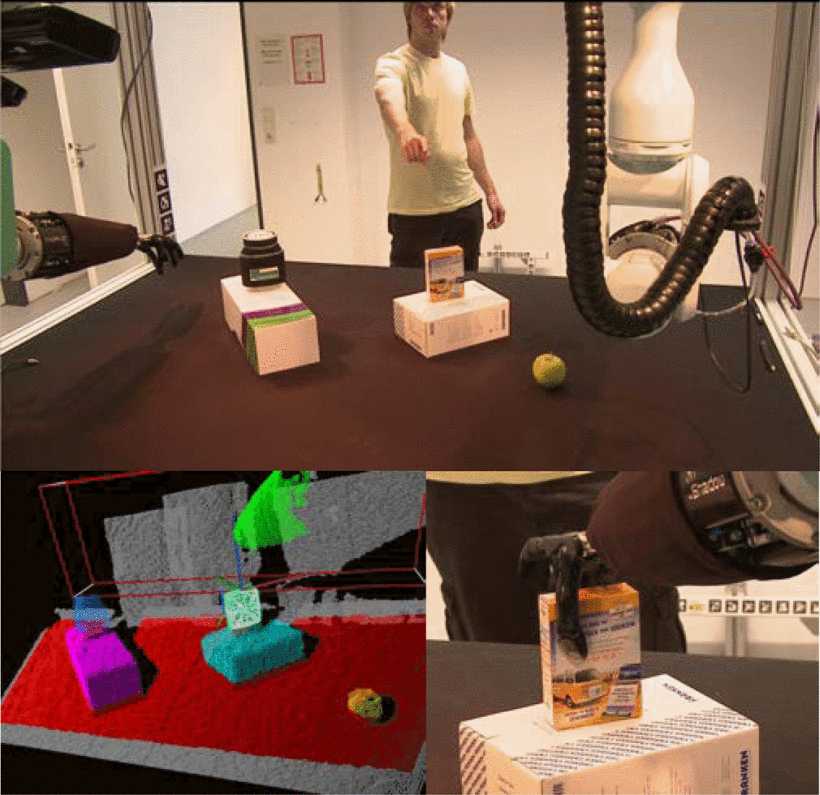
\includegraphics[height=0.7\textheight]{figures/3d_semantic_grasping.png}
%    \end{figure}
%\footcitetext{6385692}
%\end{frame}

\begin{frame}{Introduction}
    

    \begin{itemize}
        \item Grasping of moving object is one of important operations for modern robots.
        \item Objects have to be \textbf{detected} and \textbf{localized}.
        \item Semantic segmentation can be used $\rightarrow$ Multiple instances of same class can not be distinguished.
    \end{itemize}
    $\Rightarrow $ Are state of the art instance segmentation algorithms viable for real-time applications ?
    
\end{frame}

\section{State of the Art}

\subsection{Semantic Segmentation}
\begin{frame}{Semantic Segmentation}
\begin{columns}
    \begin{column}{0.5\textwidth}
        \begin{itemize}
            \item Every Pixel is labeled.
            \item Instances of the same class \textbf{can not be distinguished}.
            \item Decoder-encoder architecture.
            \item Commonly used architectures:
            \begin{itemize}
                \item DeepLabV3~\footnotemark
                
                \item SegNet~\footnotemark
                
            \end{itemize}
        \end{itemize}
    \end{column}
    \begin{column}{0.5\textwidth}
        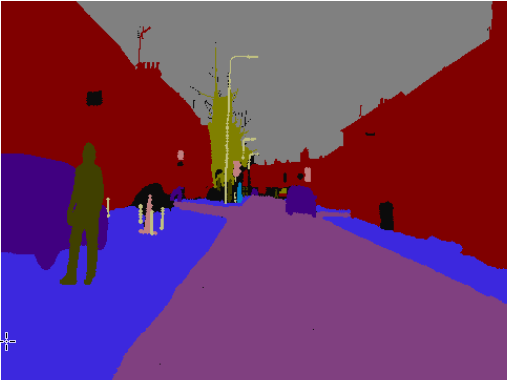
\includegraphics[width=\textwidth]{figures/segnet_example.png}
    \end{column}
\end{columns}
\footcitetext{DBLP:journals/corr/abs-1802-02611}
\footcitetext{DBLP:journals/corr/BadrinarayananK15}
\end{frame}


\subsection{Instance Segmentation}
\begin{frame}{Instance Segmentation}
    \begin{columns}
        \begin{column}{0.5\textwidth}
           \begin{itemize}
               \item Every Pixel is labeled.
               \item Different instances of the same class \textbf{are separated}.
               \item More complex pipelines.
               \item Commonly used architectures:
               \begin{itemize}
                   \item Mask R-CNN~\footnotemark
                   \item Hybrid Task Cascade~\footnotemark
                   \item ESE-Seg~\footnotemark
               \end{itemize}
           \end{itemize}
        \end{column}
        \begin{column}{0.5\textwidth}
            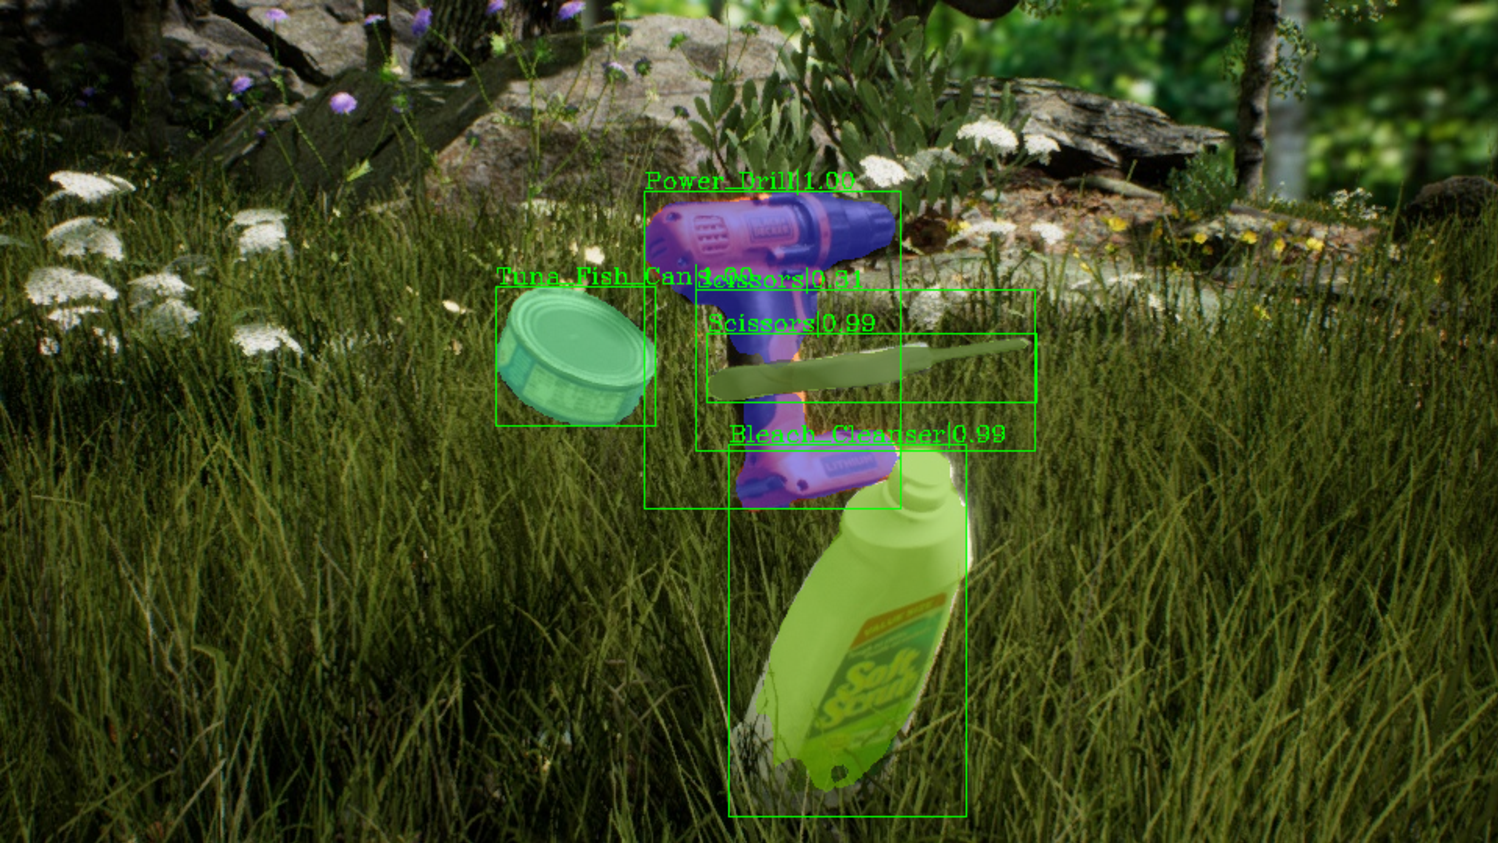
\includegraphics[width=\textwidth]{figures/cmrcnn_mobilenet_fat.pdf}
        \end{column}
\end{columns}
\footcitetext{DBLP:journals/corr/HeGDG17}
\footcitetext{DBLP:journals/corr/abs-1901-07518}
\footcitetext{2019arXiv190804067X}
\end{frame}

\subsection{Datasets}

\begin{frame}{Datasets}
\begin{itemize}
    \item Common Objects in Context (COCO)
    \begin{itemize}
        \item 115 000 annotated images.
        \item Indoor and outdoor scenes.
        \item 80 foreground object classes.
    \end{itemize}
    \item Falling Things Dataset (FAT)
    \begin{itemize}
        \item 60 000 annotated images.
        \item Synthetic dataset.
        \item Objects failing through synthetic backgrounds.
    \end{itemize}
    \item YCB Video Dataset (YCB)
    \begin{itemize}
        \item 12 000 annotated images.
        \item Video frames from a camera pan around objects.
        \item Same objects as in the FAT dataset.
    \end{itemize}
\end{itemize}
\end{frame}

\begin{frame}{COCO Dataset}
\centering
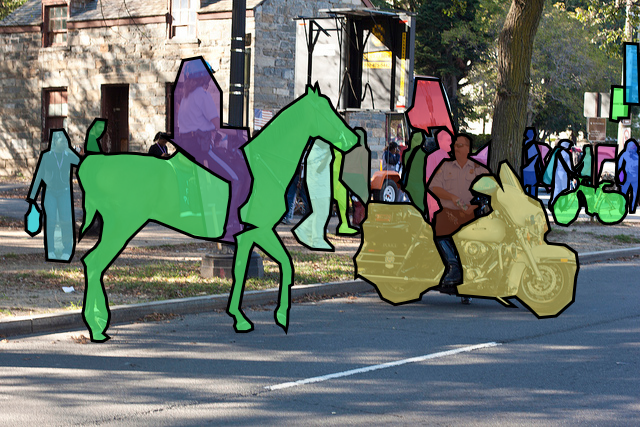
\includegraphics[height=0.8\textheight]{figures/coco_example_outdoor.png}
\end{frame}

\begin{frame}{FAT \& YCB Video Dataset}
\begin{columns}
\begin{column}{0.5\textwidth}
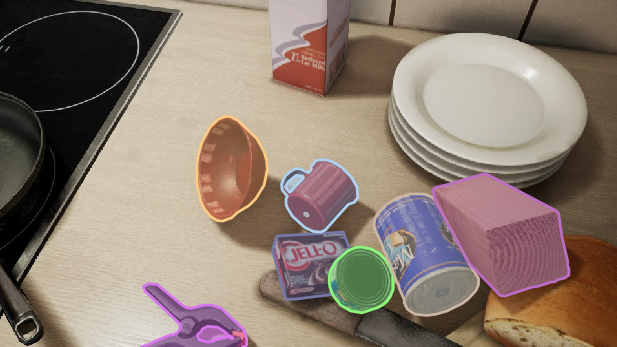
\includegraphics[width=\textwidth]{figures/fat_example_ann_3.png}
\end{column}
\begin{column}{0.5\textwidth}
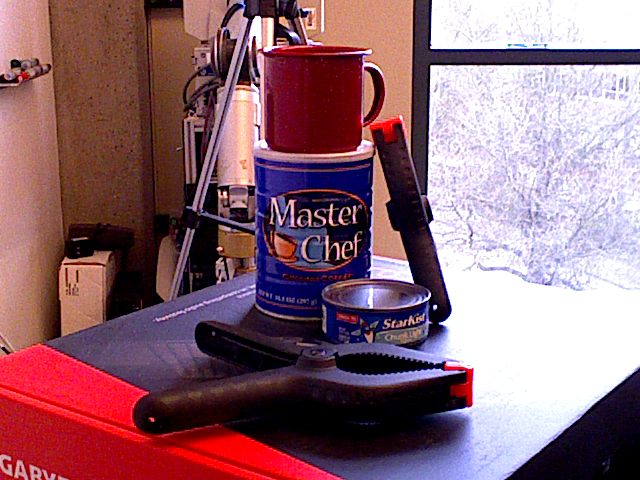
\includegraphics[width=\textwidth]{figures/ycb_video.jpg}
\end{column}
\end{columns}

\end{frame}

\section{Objectives}
\begin{frame}{Objectives}
\begin{itemize}
    \item Analysis of state of the art instance segmentation algorithms for real-time applications.
    \item Analysis of the \textbf{generalization} of such networks and the tradeoff between result \textbf{quality} and \textbf{processing times}.
\end{itemize}
\end{frame}

\section{Method}
\begin{frame}
\vfill
\centering
{\LARGE Method}
\vfill
\end{frame}

\begin{frame}{Method}
\begin{itemize}
	\item Analysis and evaluation of two state of the art neural nerworks for instance segmentation:
	\begin{itemize}
		\item YOLACT - You Only Look at Coefficients
		\item CMRCNN - Cascade Mask R-CNN
	\end{itemize}
	\item Each network was tested with multiple backbones.
    \item Different datasets were used:
    \begin{itemize}
        \item COCO Dataset
        \item FAT Dataset (Synthetic) 
        \item YCB Video Dataset (Real)
    \end{itemize}
\end{itemize}
\end{frame}

\subsection{Neural Network Architectures}
\begin{frame}{Neural Network Architectures}
\centering
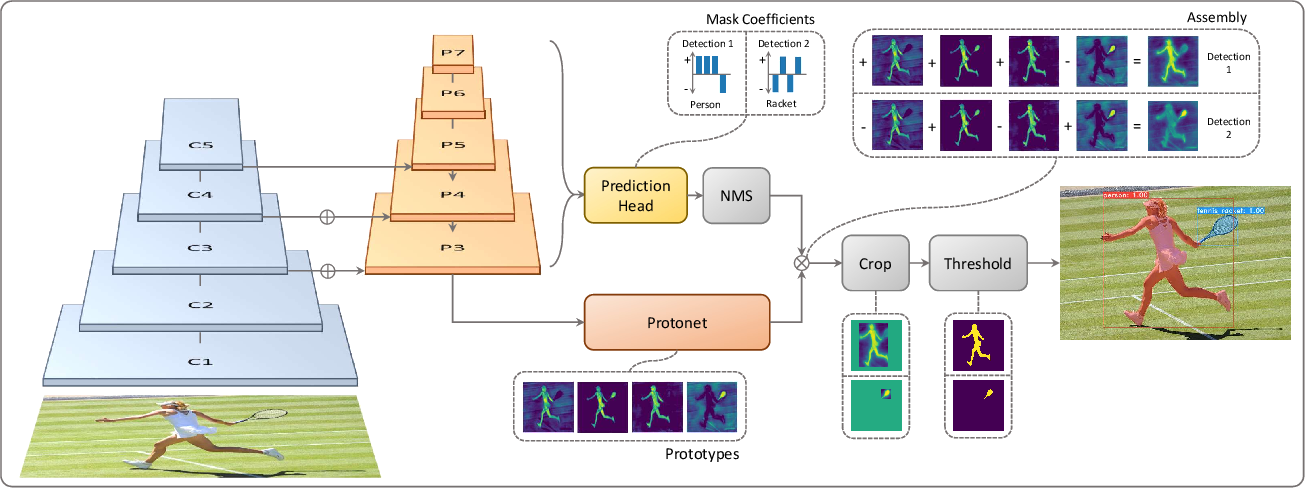
\includegraphics[height=0.45\textheight]{figures/yolact_architecture.png}
\begin{block}{YOLACT~\footnotemark~- You Only Look at Coefficients}
	\begin{itemize}
		\item Processing \textbf{time} optimized architecture.
		\item Splits information flow into two branches.
		\begin{itemize}
			\item \textbf{Mask part predictions} for all possible objects.
			\item \textbf{Coefficients} for a mask part prediction to belong to a class instance.
		\end{itemize}
	\end{itemize}
\end{block}
\footcitetext{Bolya:2019aa}
\end{frame}

\begin{frame}{Neural Network Architectures}
\centering
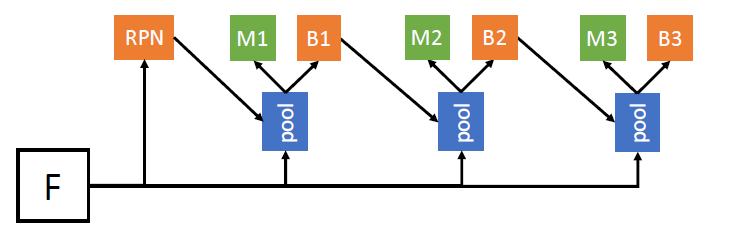
\includegraphics[height=0.45\textheight]{figures/cascade_mask_r-cnn_architecture.png}
\begin{block}{CMRCNN~\footnotemark~- Cascade Mask R-CNN}
	\begin{itemize}
		\item \textbf{Quality} optimized architecture.
		\item Based on  the Mask R-CNN architecture.
		\item Slower processing times.
	\end{itemize}
\end{block}
\footcitetext{DBLP:journals/corr/abs-1712-00726}
\end{frame}



\subsection{Metrics}

\begin{frame}{Average Precision (AP) \& \\ Average Recall (AR)}
	\begin{block}{Average Precision}
		\begin{itemize}
			\item Precision is defined as the fraction of all \textbf{correctly localized} and \textbf{classified} detections in \textbf{all correctly localized} detections.
			\item Represents the average quality of the detections over all images.
		\end{itemize}
	\end{block}
	\begin{block}{Average Recall}
		\begin{itemize}
			\item Recall is defined as the fraction of all \textbf{correctly localized} and \textbf{classified} detections in \textbf{all correctly classified} detections.
			\item Represents the average fraction of correctly predicted objects.
		\end{itemize}
	\end{block}
\end{frame}

\begin{frame}{Processing Times}
	\begin{itemize}
		\item Processing Time analysis allows to estimate the throughput of a network under certain conditions.
		\item Measuring the time between the predictions for consecutive frames for 30 minutes.
		\item Evaluated for two different system conditions:
        \begin{itemize}
            \item \textbf{average} case
            \item \textbf{worst} case 
        \end{itemize}
	\end{itemize}
\end{frame}

\begin{frame}{Processing Times}
\begin{block}{Average Case Processing Time}
	\begin{itemize}
		\item The system was in a \textbf{idle} state. There were no other foreground programs running.
		\item The GPU was not used by any other program during the test.
	\end{itemize}
\end{block}
\pause
\begin{block}{Worst Case Processing Time}
	\begin{itemize}
		\item The system was in a \textbf{stressed} state.
		\item CPU, RAM and the IO bus were kept at 100\% load for the entire test.
		\item The GPU was not used by any other program during the test.
	\end{itemize}
\end{block}
\end{frame}

\section{Results}

\begin{frame}
\vfill
\centering
{\LARGE Results}
\vfill
\end{frame}

\begin{frame}{Backbone Networks}
\begin{itemize}
    \item Backbones greatly influence the quality of the masks.
\end{itemize}
\begin{table}[H]
    \centering
        \begin{tabular}{ll | ccc}
            \toprule
            Network                         & Backbone      & $AP$              & $AP_{50}$         & $AP_{75}$ \\
            \midrule
            \multirow{3}{*}{Cascade M-RCNN} & ResNet18      & 0.669 			&  0.824 &  0.726 \\
            \multirow{1}{*}{}               & ResNet50      & \textbf{0.724} 	&  \textbf{0.877} &  \textbf{0.777} \\
            \multirow{1}{*}{}               & MobileNetV2   & 0.641 			&  0.807 &  0.690 \\
            \cline{3-5}
            \multirow{2}{*}{YOLACT}         & ResNet50      &  0.559 			&  0.712 &  0.616  \\
            \multirow{1}{*}{}               & MobileNetV2   &  0.279 			&  0.439 &  0.289  \\
            \bottomrule
        \end{tabular}
\end{table}
\end{frame}

\begin{frame}{Generalization}
\begin{itemize}
    \item The evaluated architectures \textbf{do not generalize} well from synthetic to real data.
\end{itemize}
\centering 
{\small FAT Dataset (synthetic):}
\begin{table}[H]
    \centering
    \resizebox{!}{0.15\textheight}{%
    \begin{tabular}{ll | ccc}
        \toprule
        Network                         & Backbone      & $AP$              & $AP_{50}$         & $AP_{75}$ \\
        \midrule
        \multirow{3}{*}{Cascade M-RCNN} & ResNet18      & 0.669 			&  0.824 &  0.726 \\
        \multirow{1}{*}{}               & ResNet50      & \textbf{0.724} 	&  \textbf{0.877} &  \textbf{0.777} \\
        \multirow{1}{*}{}               & MobileNetV2   & 0.641 			&  0.807 &  0.690 \\
        \cline{3-5}
        \multirow{2}{*}{YOLACT}         & ResNet50      &  0.559 			&  0.712 &  0.616  \\
        \multirow{1}{*}{}               & MobileNetV2   &  0.279 			&  0.439 &  0.289  \\
        \bottomrule
    \end{tabular}
    }
\end{table}
\centering 
{\small YCB Video Dataset (real):}
\begin{table}[H]
    \centering
    \resizebox{!}{0.15\textheight}{%
    \begin{tabular}{ll | ccc}
        \toprule
        Network                         & Backbone      & $AP$              & $AP_{50}$         & $AP_{75}$ \\
        \midrule
        \multirow{3}{*}{Cascade M-RCNN} & ResNet18      &    0.187 &  0.320 &  0.197  \\
        \multirow{1}{*}{}               & ResNet50      &     0.175 &  0.273 &  0.190 \\
        \multirow{1}{*}{}               & MobileNetV2   &     0.142 &  0.372 &  0.1388  \\
        \cline{3-5}
        \multirow{2}{*}{YOLACT}         & ResNet50      &     \textbf{0.218} &  \textbf{0.407} &  \textbf{0.228} \\
        \multirow{1}{*}{}               & MobileNetV2  	&    0.104 &  0.211 &  0.092 \\
        \bottomrule
    \end{tabular}
    }
\end{table}
\end{frame}

\begin{frame}{Segmentation Results}
\begin{itemize}
    \item Detections by Instance segmentation networks are still error prone.
\end{itemize}
\begin{columns}
    \begin{column}{0.5\textwidth}
        \centering
        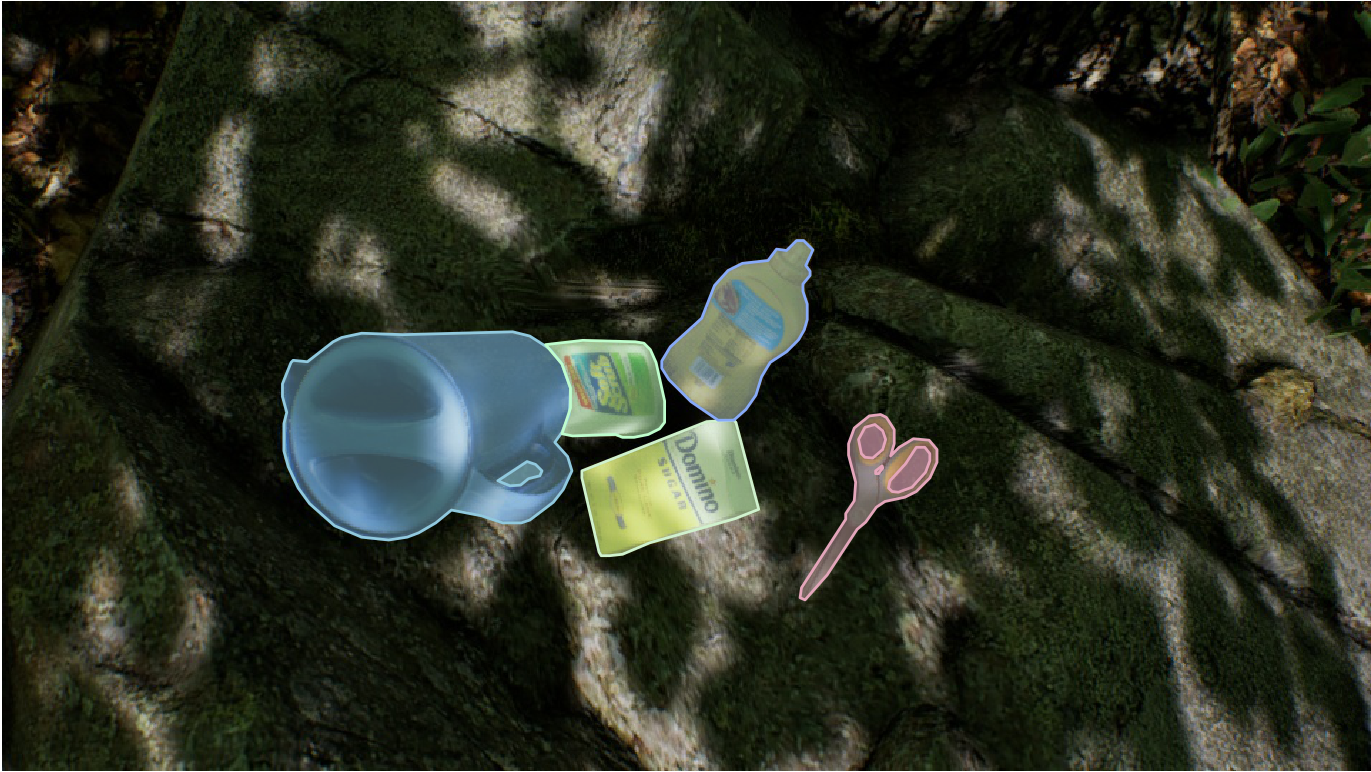
\includegraphics[width=0.8\textwidth]{figures/example_output_anns.png}
        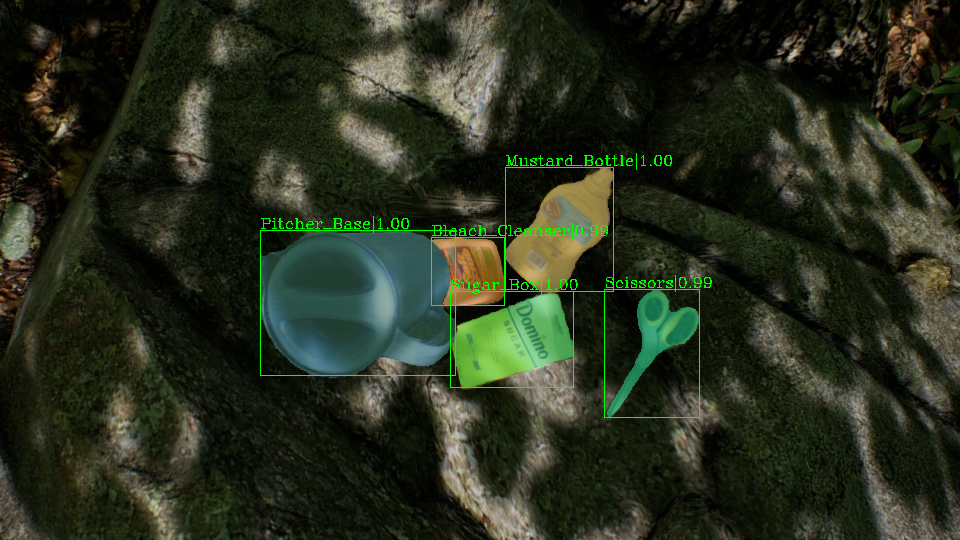
\includegraphics[width=0.8\textwidth]{figures/cmrcnn_mobilenet_fat_2.png}
        \vfill
        Valid Detection
    \end{column}
    \begin{column}{0.5\textwidth}
        \centering
    	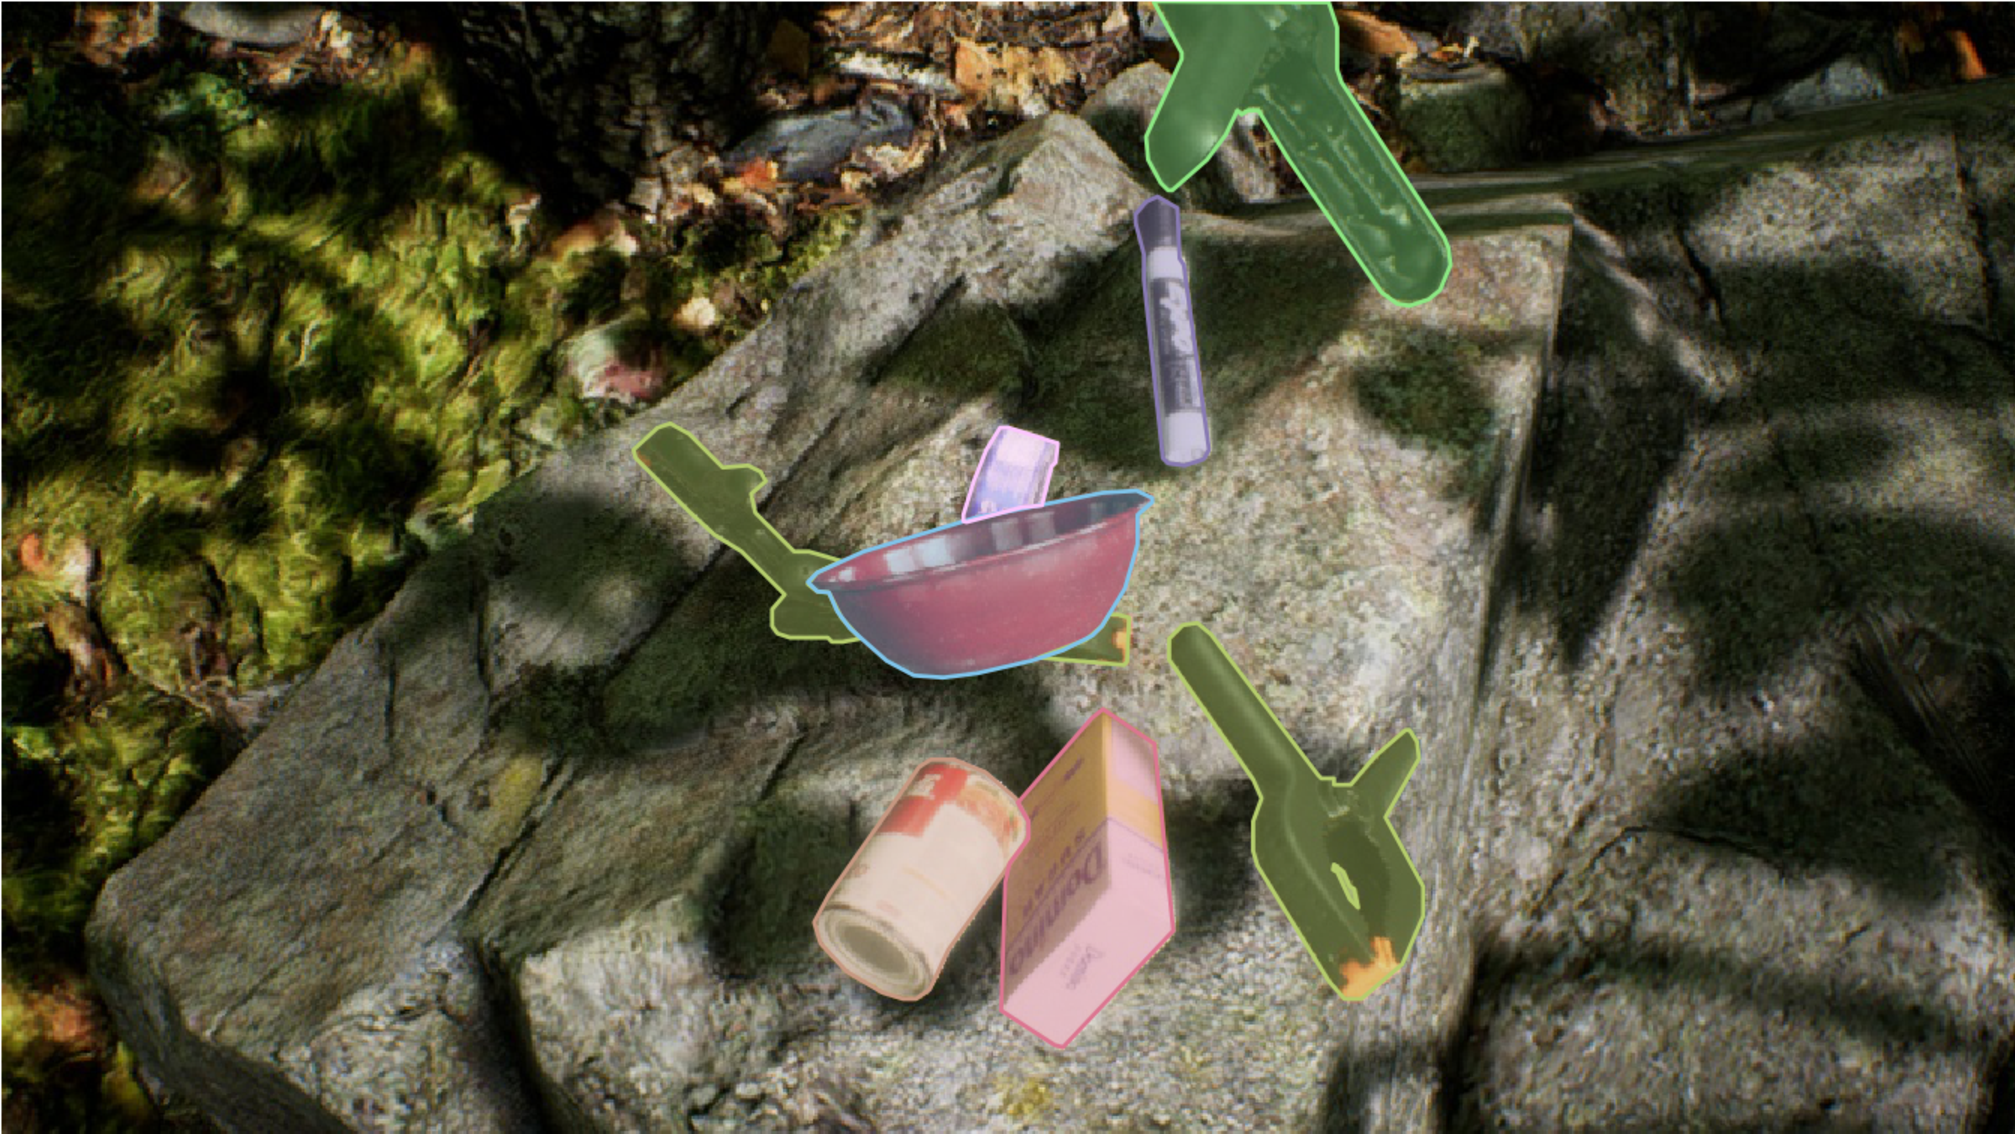
\includegraphics[width=0.8\textwidth]{figures/fat_example_ann.pdf}
        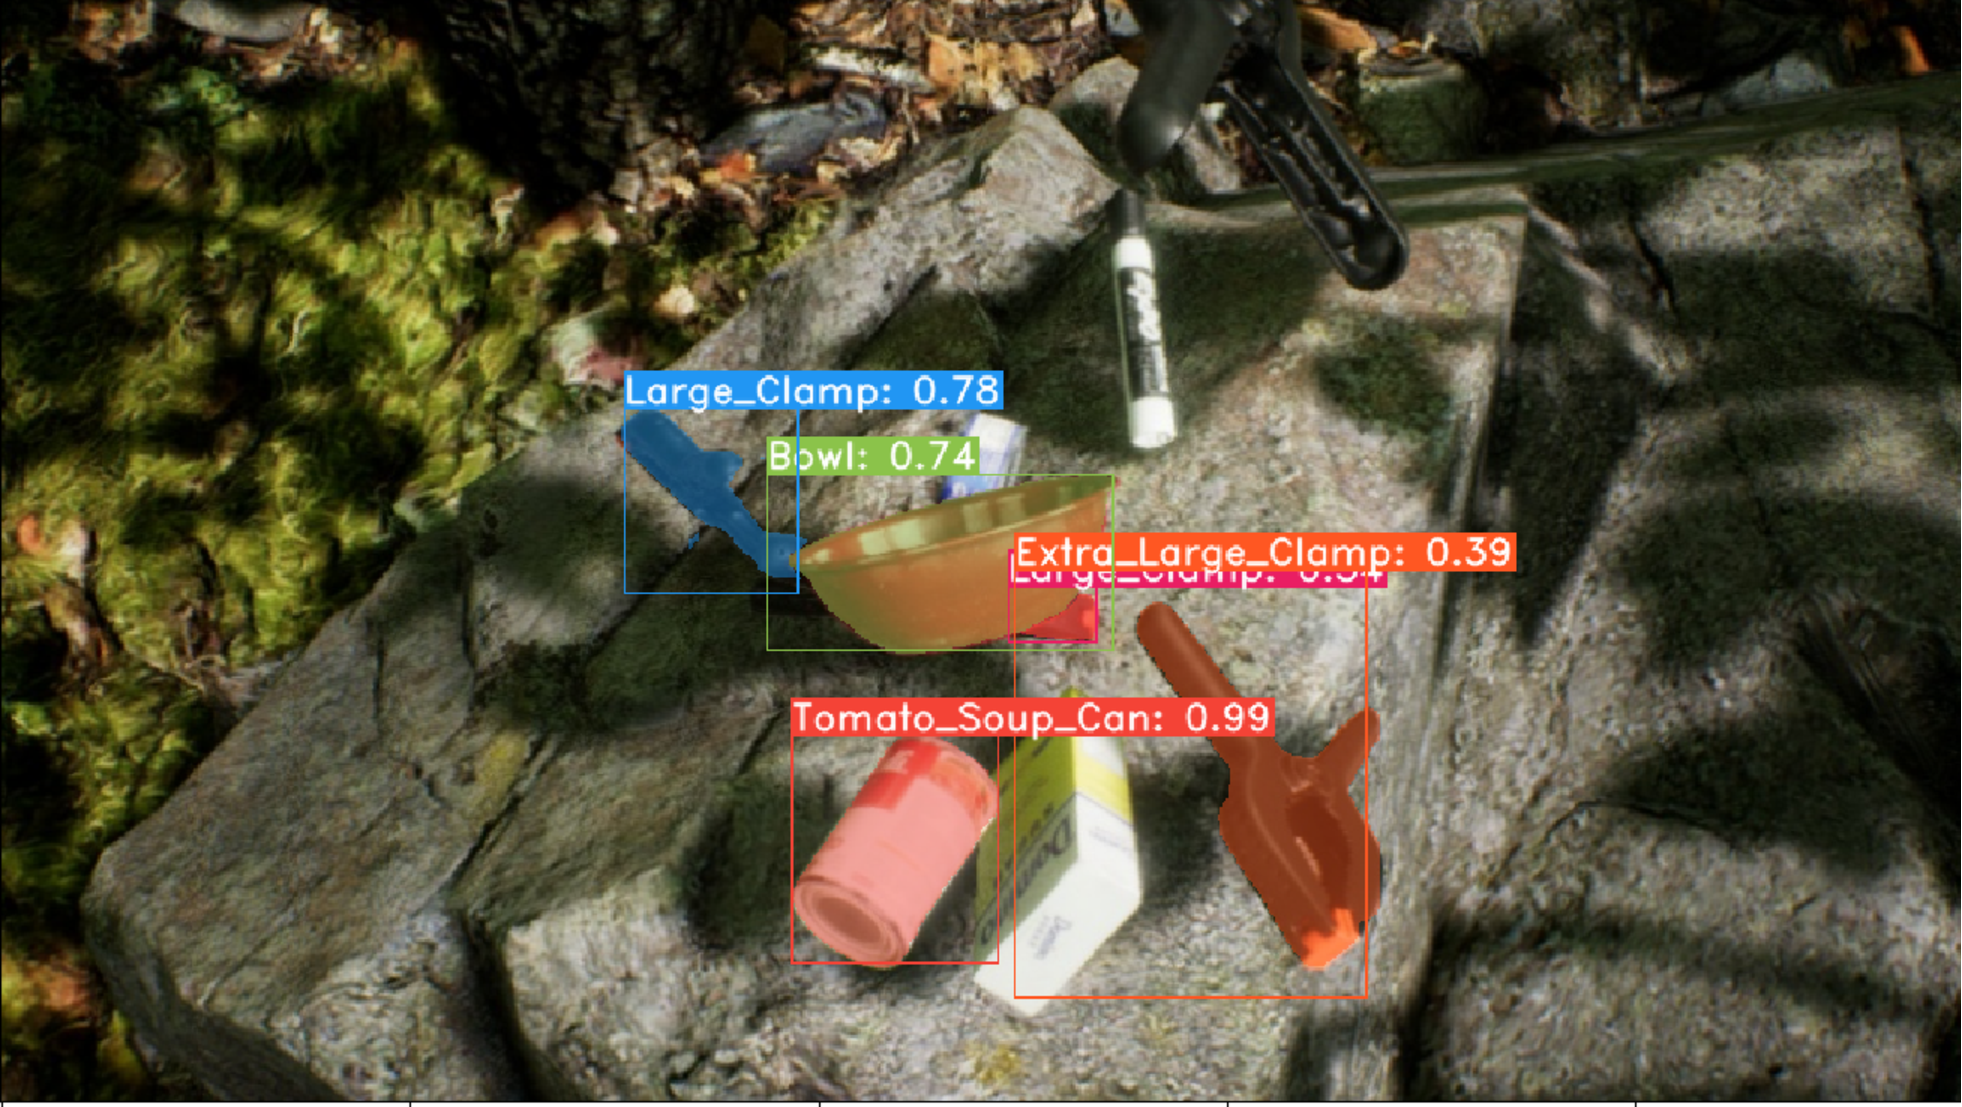
\includegraphics[width=0.8\textwidth]{figures/fat_example_invalid.pdf}
        \vfill
        Invalid Detection
    \end{column}
\end{columns}
\end{frame}

\begin{frame}{Processing Time}
    \begin{itemize}
        \item YOLACT displays fast interference time with a low variance.
    \end{itemize}
    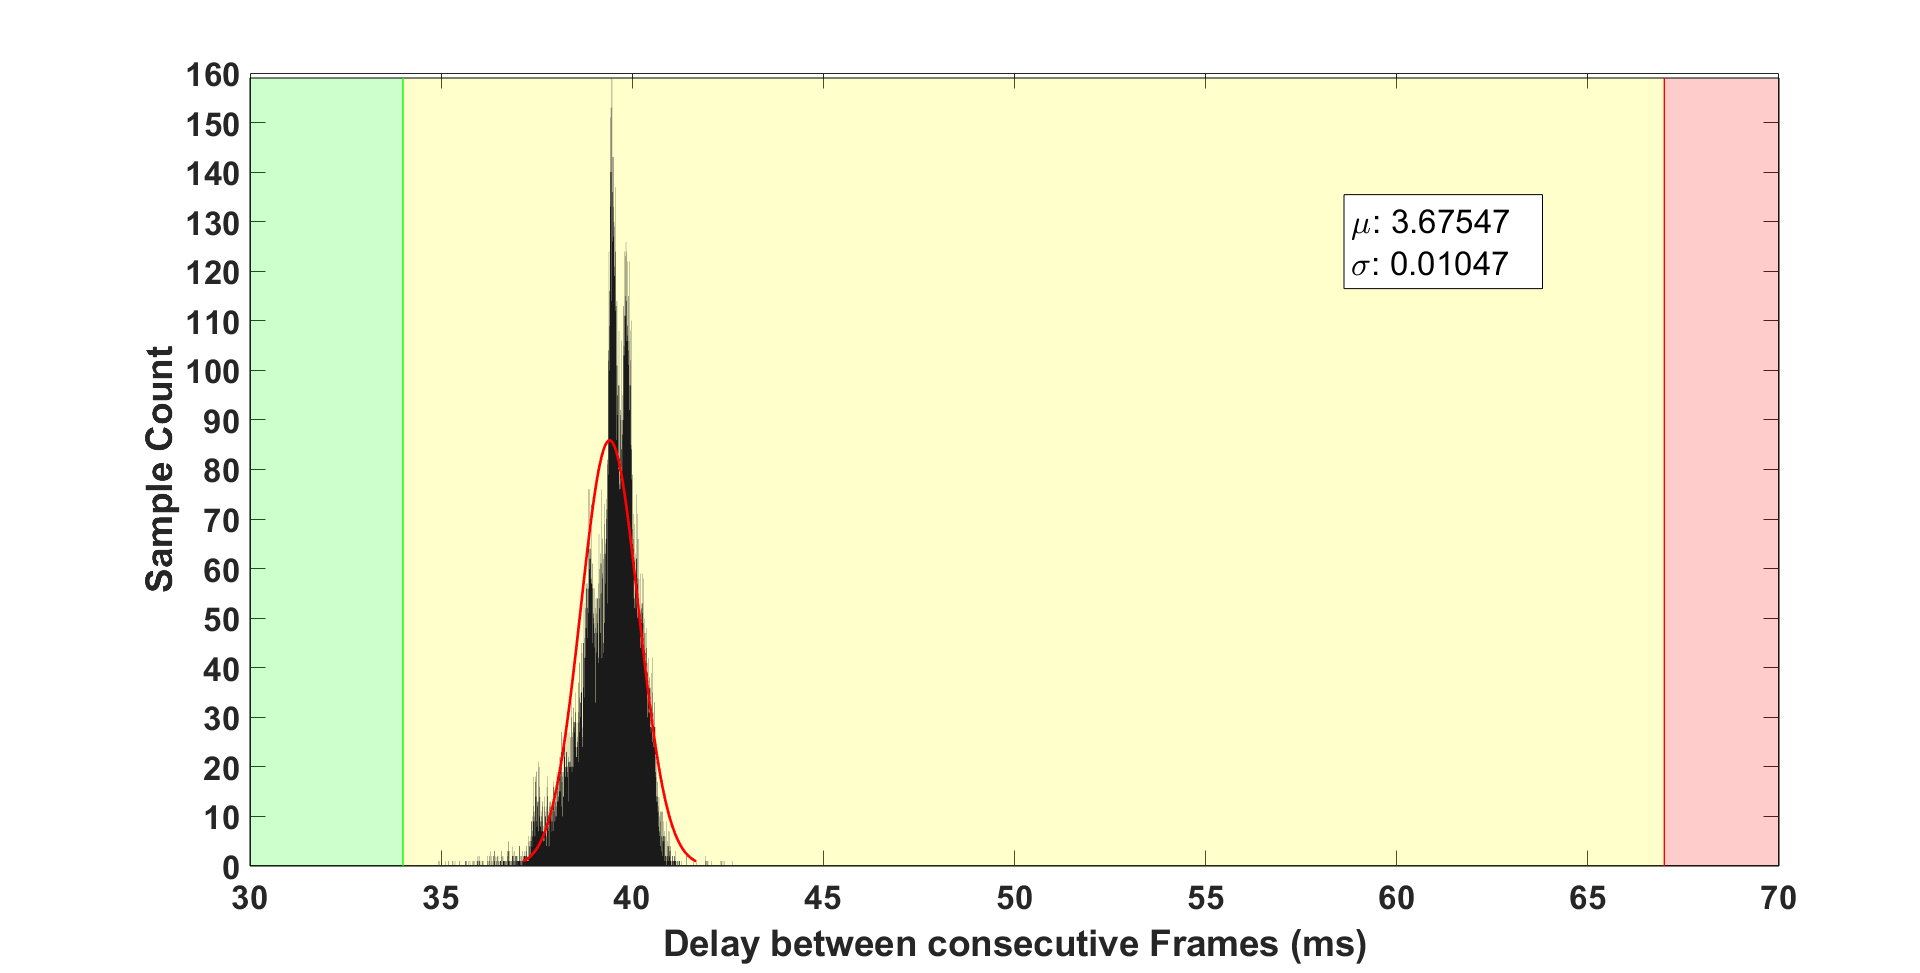
\includegraphics[width=\textwidth]{figures/graphs/dist_yolact_mobilenetv2.png}
\end{frame}

\begin{frame}{Processing Time}
    \begin{itemize}
        \item CMRCNN shows highly variant, long processing times.
    \end{itemize}
    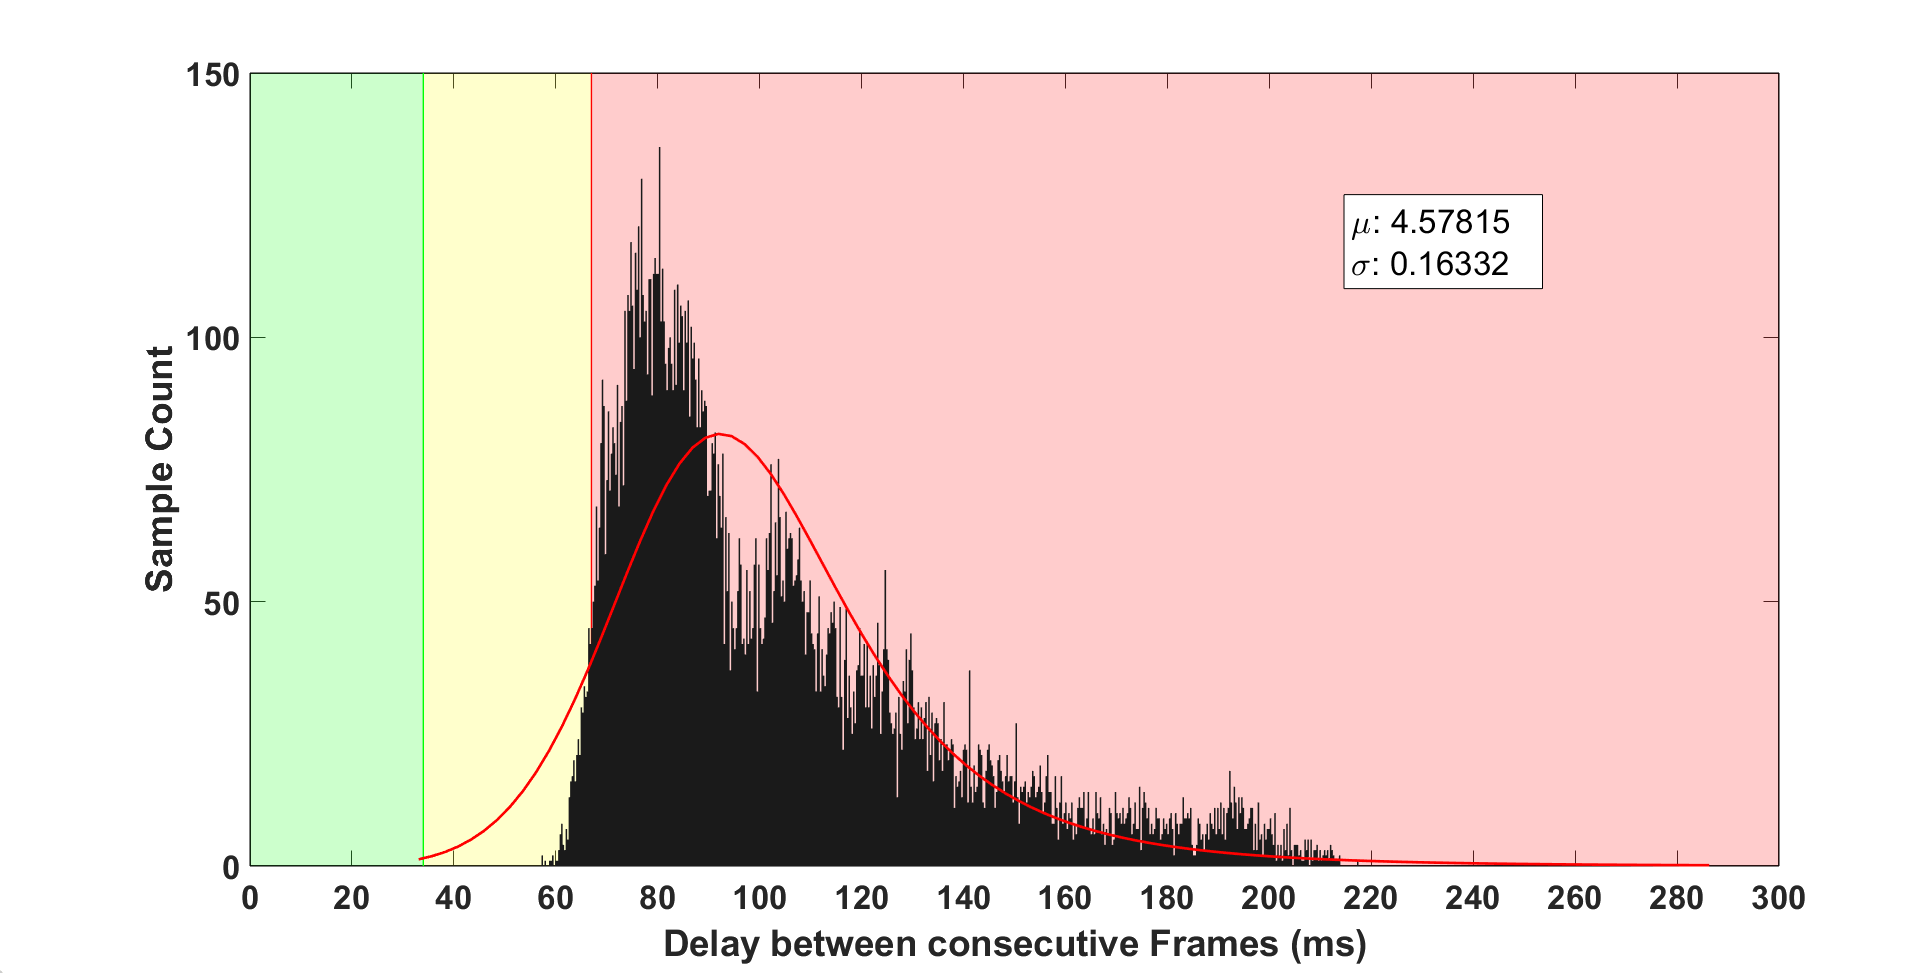
\includegraphics[width=\textwidth]{figures/graphs/dist_cmrcnn_mobilenetv2.png}
\end{frame}

\begin{frame}{Processing Time (Stress)}
\begin{itemize}
    \item Processing times are highly dependent system load.
\end{itemize}
    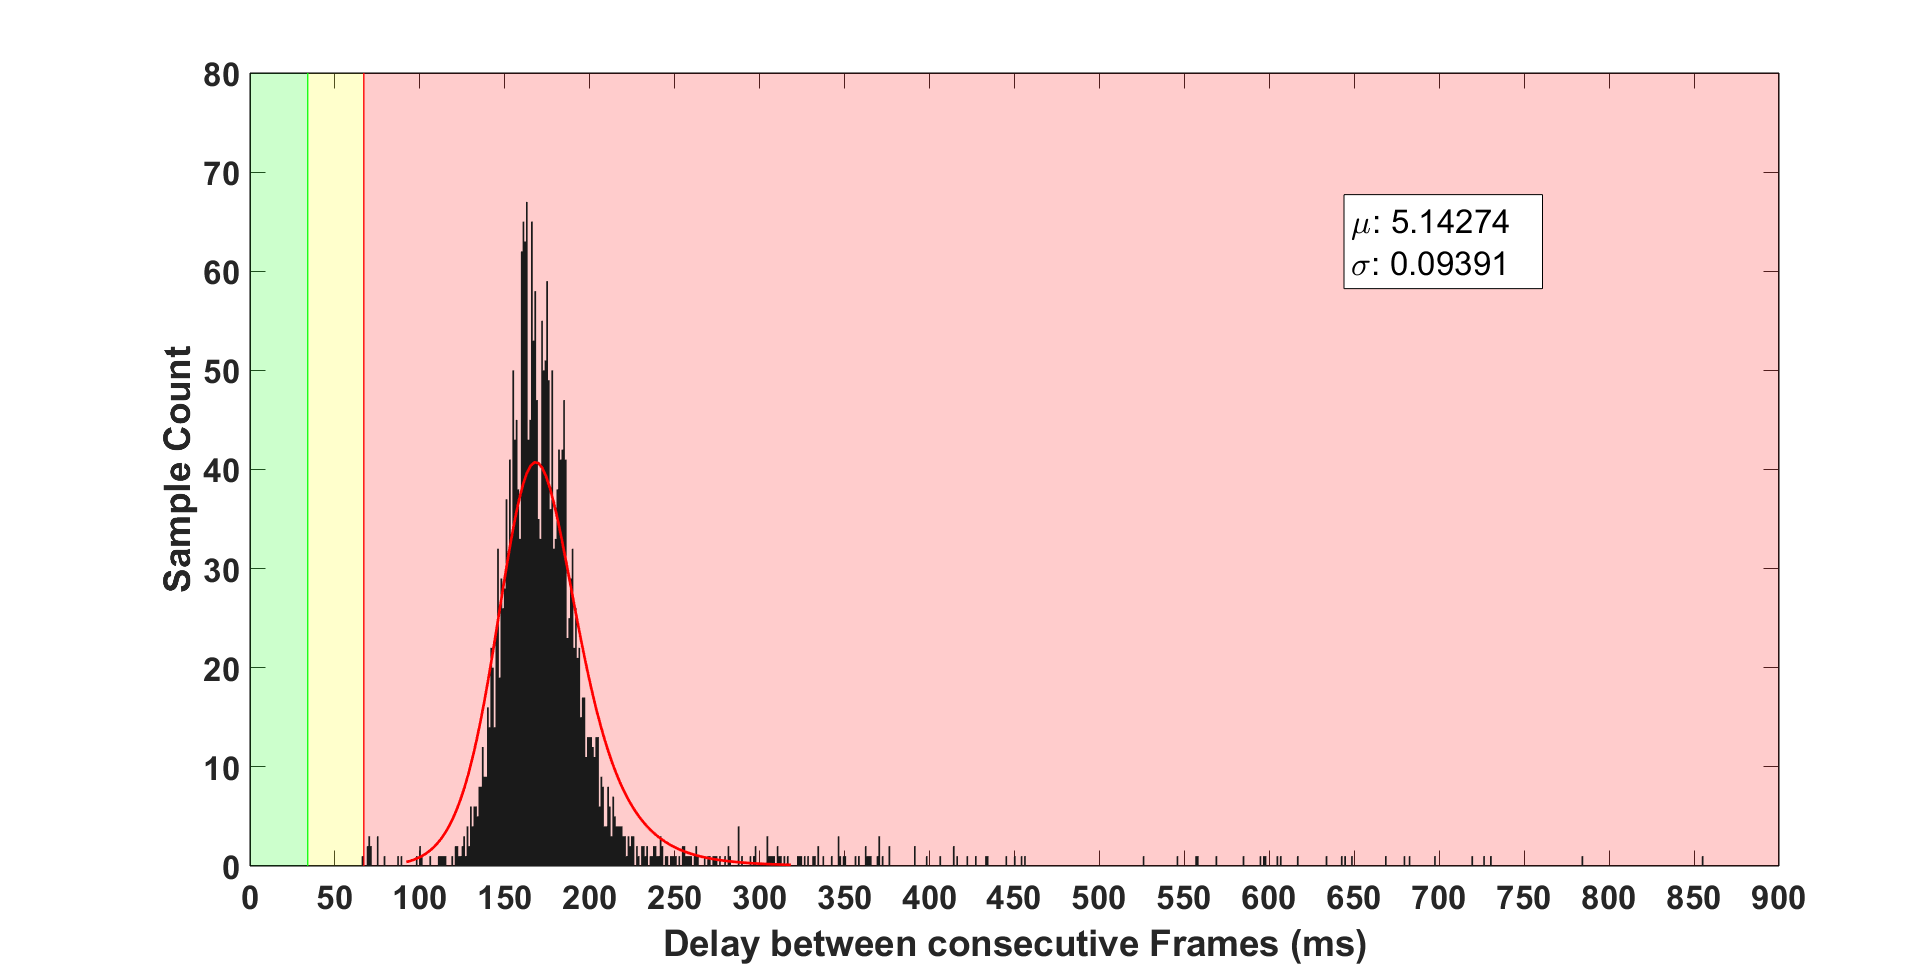
\includegraphics[width=\textwidth]{figures/graphs/dist_stress_yolact_mobilenetv2.png}
\end{frame}

\begin{frame}{Processing Time}
\begin{itemize}
    \item Computational intensive network parts determine the processing time.
\end{itemize}
\begin{columns}
    \begin{column}{0.5\textwidth}
        \centering
        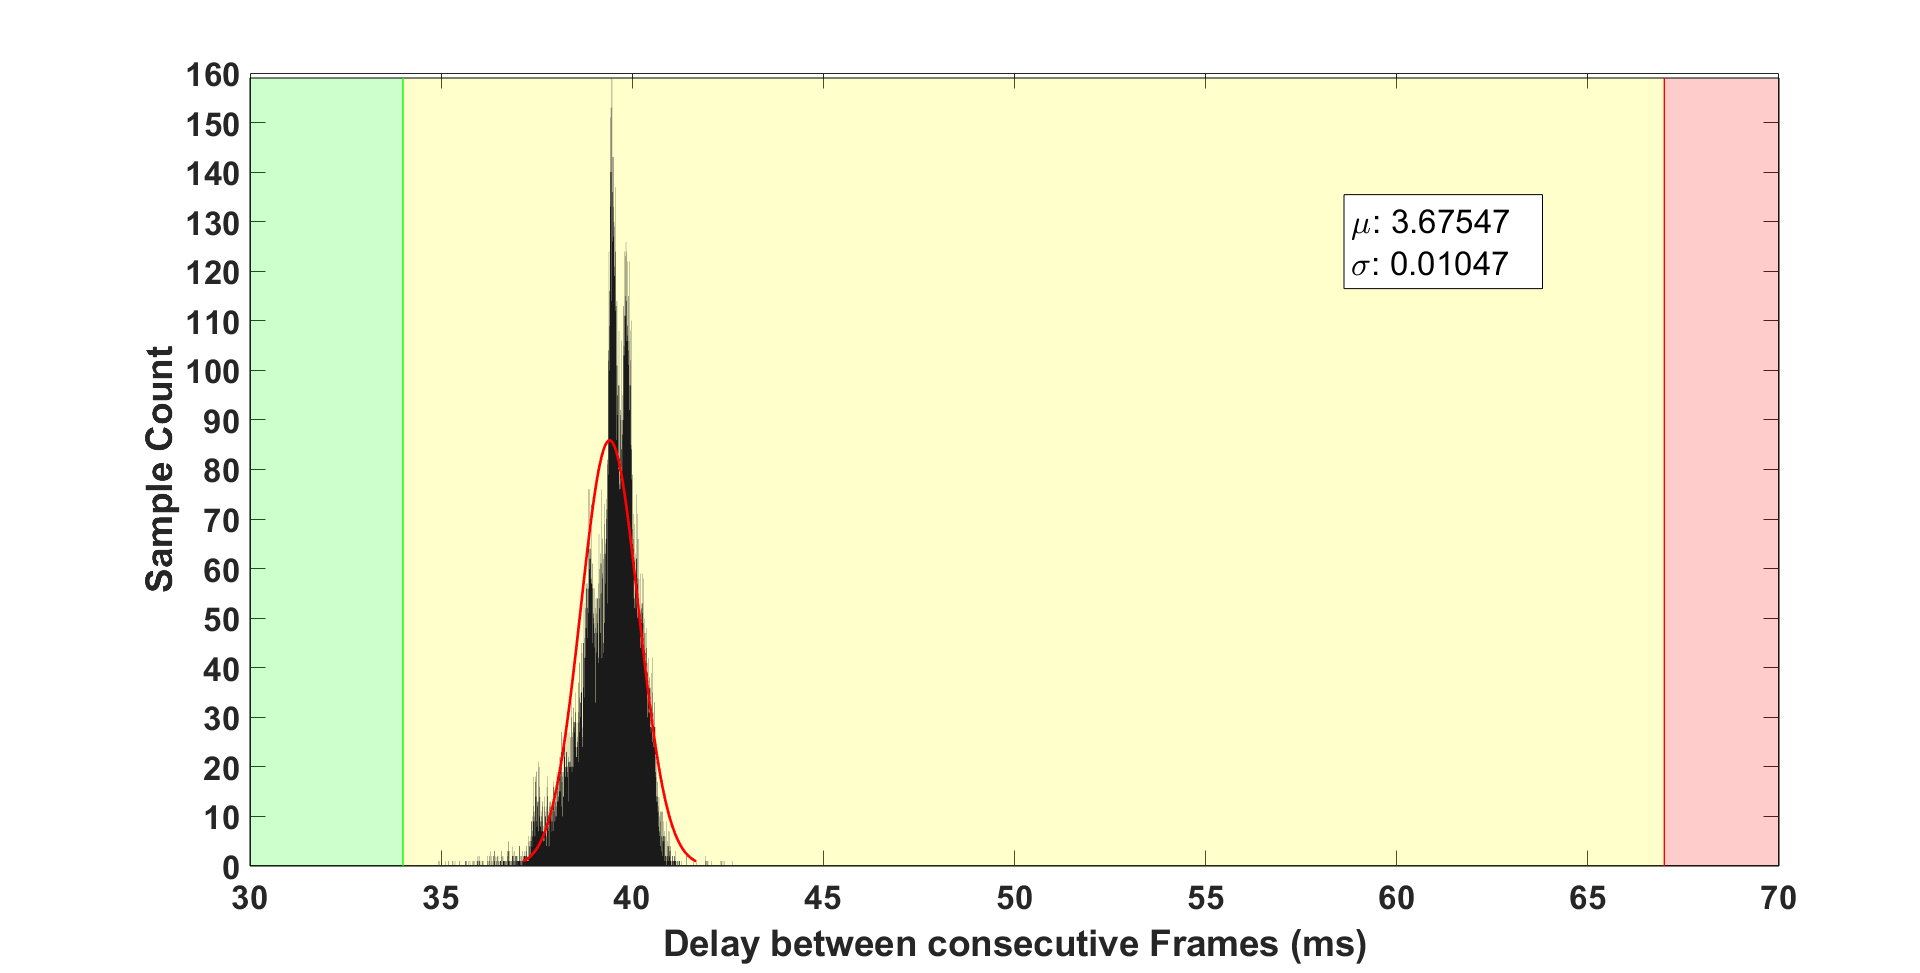
\includegraphics[width=\textwidth]{figures/graphs/dist_yolact_mobilenetv2.png}
        \vfill
        YOLACT MobileNetV2
        \vfill
    \end{column}
    \begin{column}{0.5\textwidth}
        \centering
        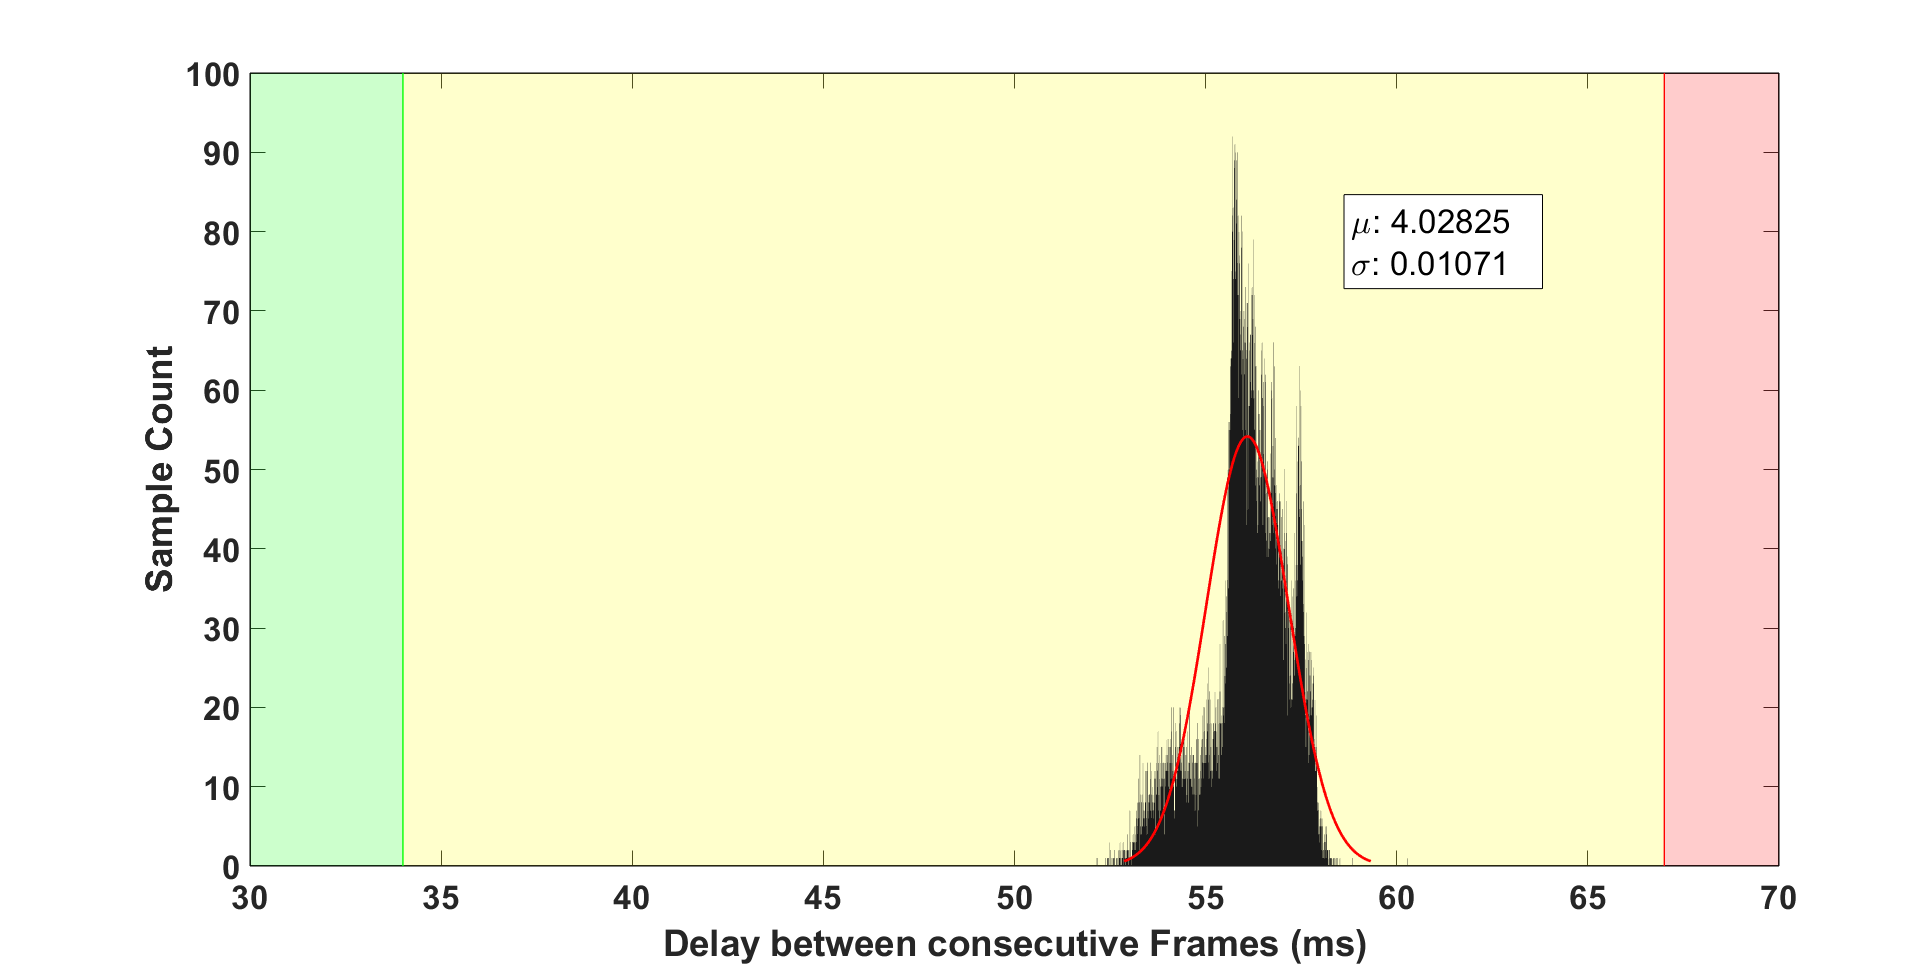
\includegraphics[width=\textwidth]{figures/graphs/dist_yolact_resnet50.png}
        \vfill
        YOLACT ResNet50
        \vfill
    \end{column}
\end{columns}
\end{frame}

\section{Conclusions}
\begin{frame}{Conclusions}

\begin{block}{Processing Time Profiling}
	\begin{itemize}
		\item Processing time is strongly bound to the architecture.
		\item Optimizing the processing times is a important topic for modern architectures.
	\end{itemize}
\end{block}
\pause
\begin{block}{Household Object Robot Grasping}
    \begin{itemize}
        \item Qualitative results are promising for future research.
        \item Robustness has to be improved for real world aplications.
        \item Dataset selection is relevant for result quality.
        \item When looking at functional safety, the current evaluation methods are not sufficient.
    \end{itemize}
\end{block}
\end{frame}

\begin{frame}
\vfill
\centering
{\LARGE Thank you for your attention.}\\
\vspace{1cm}
{\Large \textbf{Questions ?}}
\vfill
\end{frame}

\appendix
\beginbackup

\nocite{*}

\begin{frame}[allowframebreaks]{References}
\printbibliography
\end{frame}

\section{AP}

\begin{frame}{AP (COCO Dataset)}
\begin{table}[H]
	\centering
	\begin{tabular}{ll | ccc}
		\toprule
		Network                         & Backbone      & $AP$              & $AP_{50}$         & $AP_{75}$ \\
		\midrule
		\multirow{3}{*}{Cascade M-RCNN} & ResNet18      &  0.169 &  0.280 &  0.177 \\
		\multirow{1}{*}{}               & ResNet50      &  \textbf{0.369} &  \textbf{0.586} &  \textbf{0.397} \\
		\multirow{1}{*}{}               & MobileNetV2   &  0.167 &  0.278 &  0.174 \\
		\cline{3-5}
		\multirow{2}{*}{YOLACT}         & ResNet50      &  0.265 &  0.443 &  0.272 \\
		\multirow{1}{*}{}               & MobileNetV2   &  0.054 &  0.101 &  0.051 \\
		\midrule
		Network                         & Backbone      & $AP_{Small}$      & $AP_{Medium}$     & $AP_{Large}$ \\
		\midrule
		\multirow{3}{*}{Cascade M-RCNN} & ResNet18      &  0.056 	&      0.175 &     0.271 \\
		\multirow{1}{*}{}               & ResNet50      &  \textbf{0.196} 	&      \textbf{0.393} &     \textbf{0.488} \\
		\multirow{1}{*}{}               & MobileNetV2   &  0.057 	&      0.170 &     0.276 \\
		\cline{3-5}
		\multirow{2}{*}{YOLACT}         & ResNet50      &  0.085 	&      0.289 &     0.433 \\
		\multirow{1}{*}{}               & MobileNetV2   &  0.000 	&      0.028 &     0.134 \\
		\bottomrule
	\end{tabular}
\end{table}
\end{frame}

\begin{frame}{AP (COCO 0.02 Dataset)}
\begin{table}[H]
    \centering
    \begin{tabular}{ll | ccc}
        \toprule
        Network                                           & Backbone          & $AP$                    & $AP_{50}$         & $AP_{75}$ \\
        \midrule
        \multirow{3}{*}{Cascade M-RCNN}   & ResNet18          &  0.087 &  0.133 &  0.09 \\
        \multirow{1}{*}{}                               & ResNet50          & \textbf{0.385} &  \textbf{0.542} &  \textbf{0.417} \\
        \multirow{1}{*}{}                               & MobileNetV2     &  0.327 &  0.482 &  0.350\\
        \cline{3-5}
        \multirow{2}{*}{YOLACT}         & ResNet50     &  0.374 &  0.549 &  0.401 \\
        \multirow{1}{*}{}               & MobileNetV2   &  0.059 &  0.120 &  0.051 \\
        \midrule
        Network                         & Backbone      & $AP_{Small}$      & $AP_{Medium}$     & $AP_{Large}$ \\
        \midrule
        \multirow{3}{*}{Cascade M-RCNN} & ResNet18      &     0.008 &      0.044 &     0.109 \\
        \multirow{1}{*}{}               & ResNet50      &     0.013 &      0.237 &     0.418\\
        \multirow{1}{*}{}               & MobileNetV2   &   0.067 &      0.246 &     0.398  \\
        \cline{3-5}
        \multirow{2}{*}{YOLACT}         & ResNet50      &  \textbf{0.078} &      \textbf{0.281} &     \textbf{0.450 }\\
        \multirow{1}{*}{}               & MobileNetV2   &   0.000 &      0.060 &     0.071 \\
        \bottomrule
    \end{tabular}
\end{table}
\end{frame}


\begin{frame}{AP (COCO 0.10 Dataset)}
\begin{table}[H]
    \centering
    \begin{tabular}{ll | ccc}
        \toprule
        Network                         & Backbone      & $AP$              & $AP_{50}$         & $AP_{75}$ \\
        \midrule
        \multirow{3}{*}{Cascade M-RCNN} & ResNet18      &  0.311 &  0.453 &  0.338 \\
        \multirow{1}{*}{}               & ResNet50      &  0.349 &  0.504 &  0.371\\
        \multirow{1}{*}{}               & MobileNetV2   &  0.272 &  0.414 &  0.287 \\
        \cline{3-5}
        \multirow{2}{*}{YOLACT}         & ResNet50      &  \textbf{0.352} &  \textbf{0.539} &  \textbf{0.353 }\\
        \multirow{1}{*}{}               & MobileNetV2   &  0.068 &  0.169 &  0.045  \\
        \midrule
        Network                         & Backbone      & $AP_{Small}$      & $AP_{Medium}$     & $AP_{Large}$ \\
        \midrule
        \multirow{3}{*}{Cascade M-RCNN} & ResNet18      &  \textbf{0.059} &      0.228 &     \textbf{0.390}\\
        \multirow{1}{*}{}               & ResNet50      &  0.037 &      0.193 &     0.380  \\
        \multirow{1}{*}{}               & MobileNetV2   &   0.004 &      0.110 &     0.302 \\
        \cline{3-5}
        \multirow{2}{*}{YOLACT}         & ResNet50      &  0.035 &      \textbf{0.229} &     0.372  \\
        \multirow{1}{*}{}               & MobileNetV2   &  0.000 &      0.032 &     0.078  \\
        \bottomrule
    \end{tabular}
\end{table}
\end{frame}


\section{Processing Time}

\begin{frame}{Processing Times I}
\begin{table}[h]
    \begin{tabular}{ll | ccc}
        \toprule
        \multirow{2}{*}{Network}        & \multicolumn{1}{l}{\multirow{2}{*}{Backbone}}  & $Median$  & $Mean$    & $Var$    \\
        \multirow{1}{*}{}               & \multicolumn{1}{l}{\multirow{1}{*}{}}  			& $[ms]$  	& $[ms]$    & 		     \\
        \midrule
        \multirow{3}{*}{Cascade M-RCNN} & ResNet18                      & 109.65    & 119.97    & 1615.53   \\
        \multirow{1}{*}{}               & ResNet50                      & 101.43    & 112.05    & 1146.41    \\
        \multirow{1}{*}{}               & MobileNetV2                   & 93.640    & 103.927   & 1037.521 \\
        \midrule
        \multirow{2}{*}{YOLACT}         & ResNet50                      & 56.165    & 56.092    & 1.158     \\
        \multirow{1}{*}{}               & MobileNetV2                   & \textbf{39.516} & \textbf{39.408} & \textbf{0.568}  \\
        \bottomrule
    \end{tabular}
\end{table}
\end{frame}

\begin{frame}{Processing Times II}
\begin{table}[h]
    \begin{tabular}{ll | cc}
        \toprule
        \multirow{2}{*}{Network}        & \multicolumn{1}{l}{\multirow{2}{*}{Backbone}}  & $Min$     & $Max$   \\
        \multirow{1}{*}{}               & \multicolumn{1}{l}{\multirow{1}{*}{}}  			& $[ms]$    & $[ms]$   \\
        \midrule
        \multirow{3}{*}{Cascade M-RCNN} & ResNet18                      & 59.215    & 252.038 \\
        \multirow{1}{*}{}               & ResNet50                     & 65.769    & 444.265   \\
        \multirow{1}{*}{}               & MobileNetV2                   & 57.324    & 352.360  \\
        \midrule
        \multirow{2}{*}{YOLACT}         & ResNet50                      & 52.148    & 60.293   \\
        \multirow{1}{*}{}               & MobileNetV2                   & \textbf{34.941} & \textbf{42.623}  \\
        \bottomrule
    \end{tabular}
\end{table}
\end{frame}


\begin{frame}{Processing Time Distribution CMRCNN MobileNetV2}
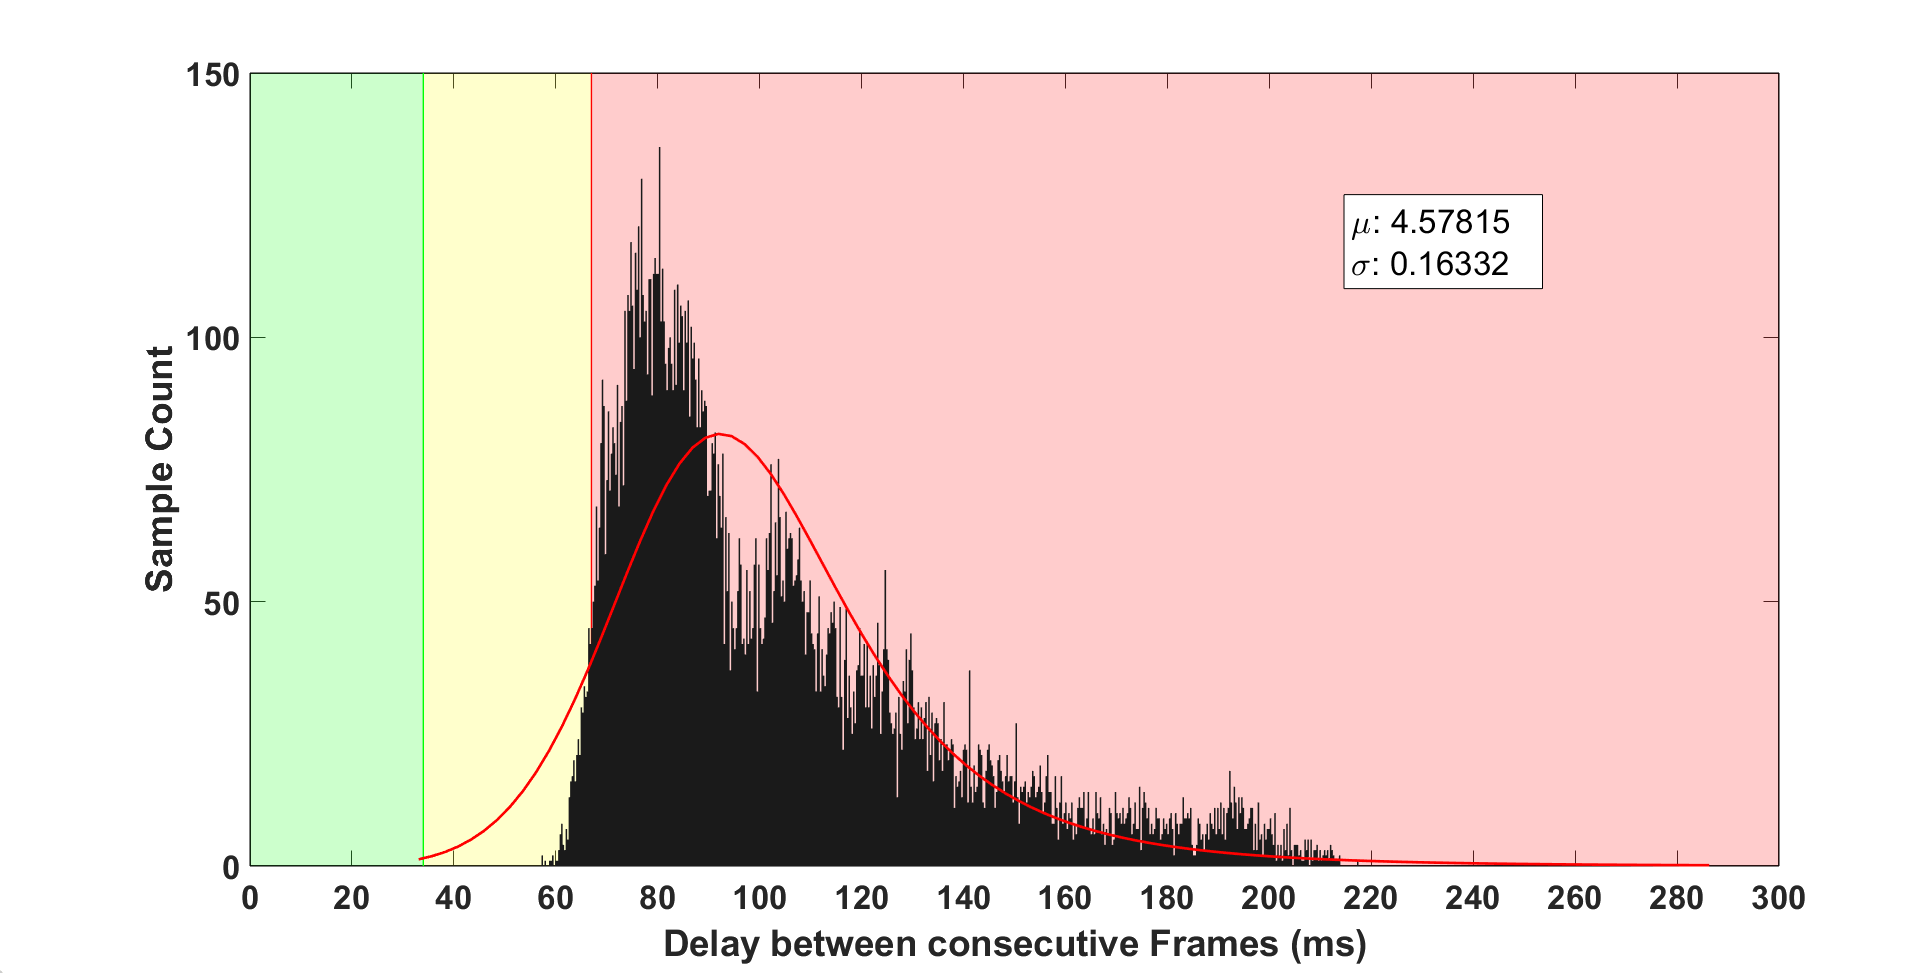
\includegraphics[width=\textwidth]{figures/graphs/dist_cmrcnn_mobilenetv2.png}
\end{frame}

\begin{frame}{Processing Time Distribution CMRCNN ResNet18}
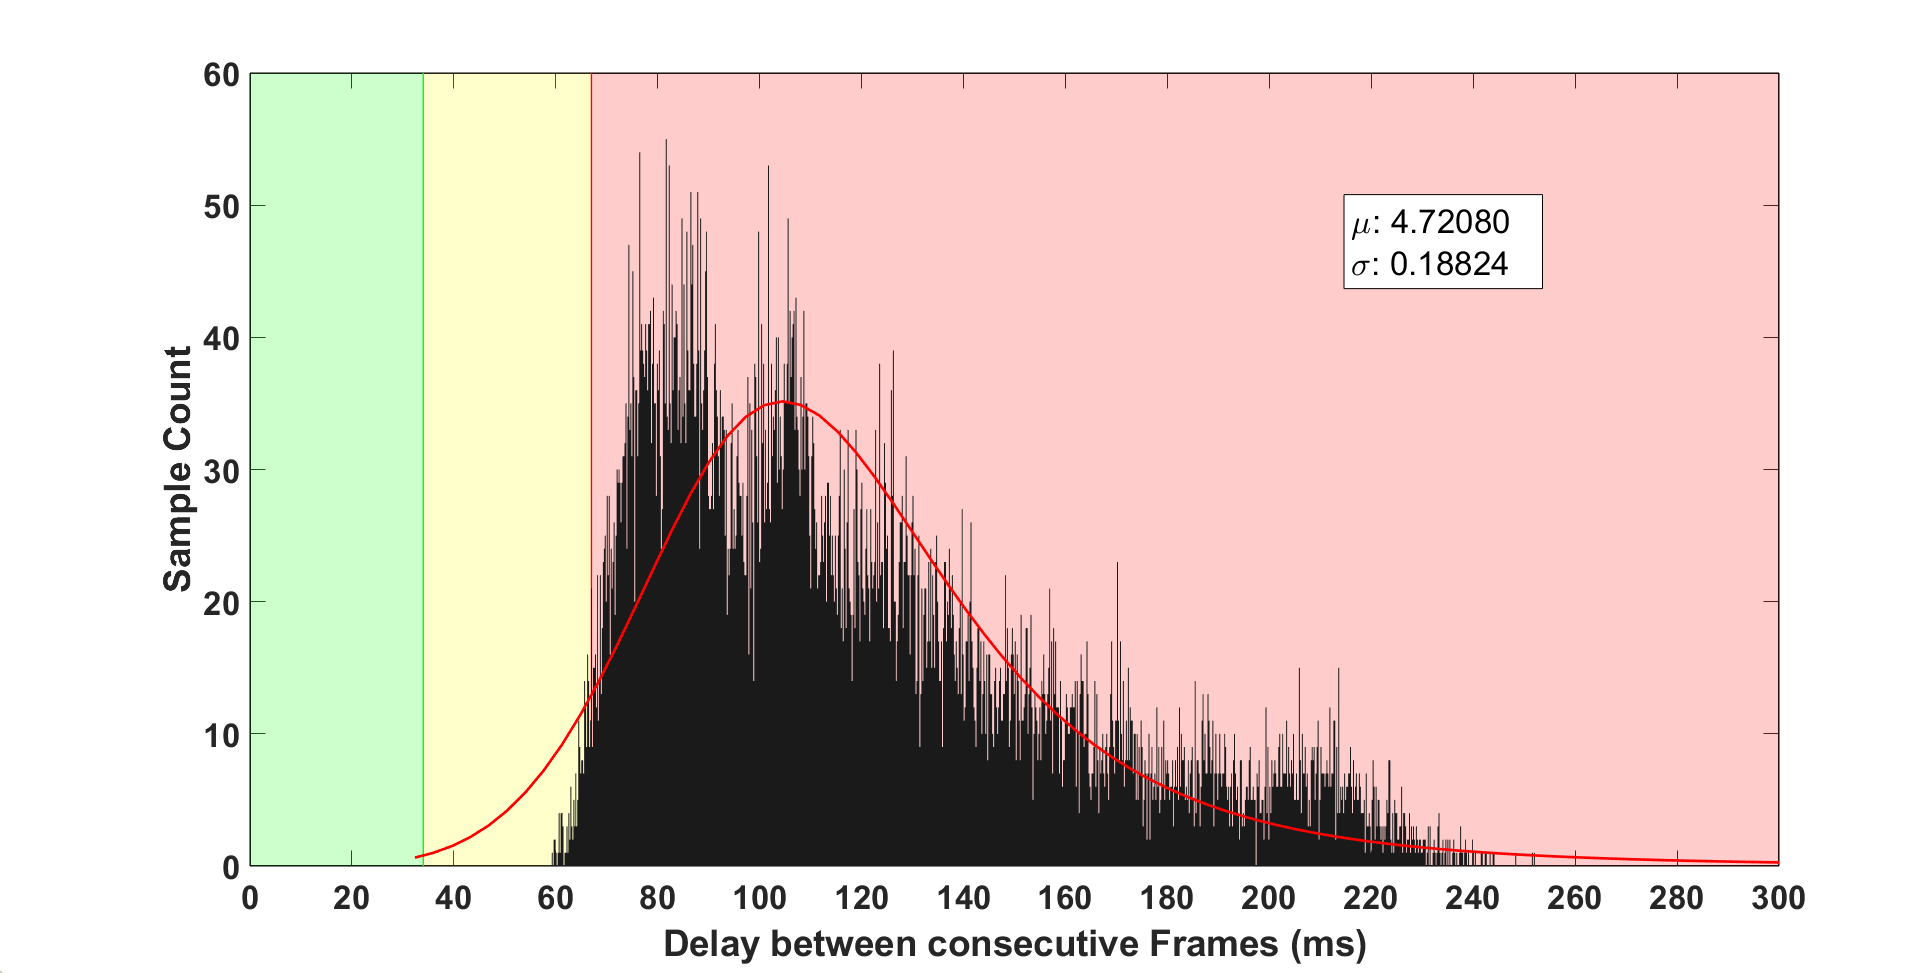
\includegraphics[width=\textwidth]{figures/graphs/dist_cmrcnn_resnet18.png}
\end{frame}

\begin{frame}{Processing Time Distribution CMRCNN ResNet50}
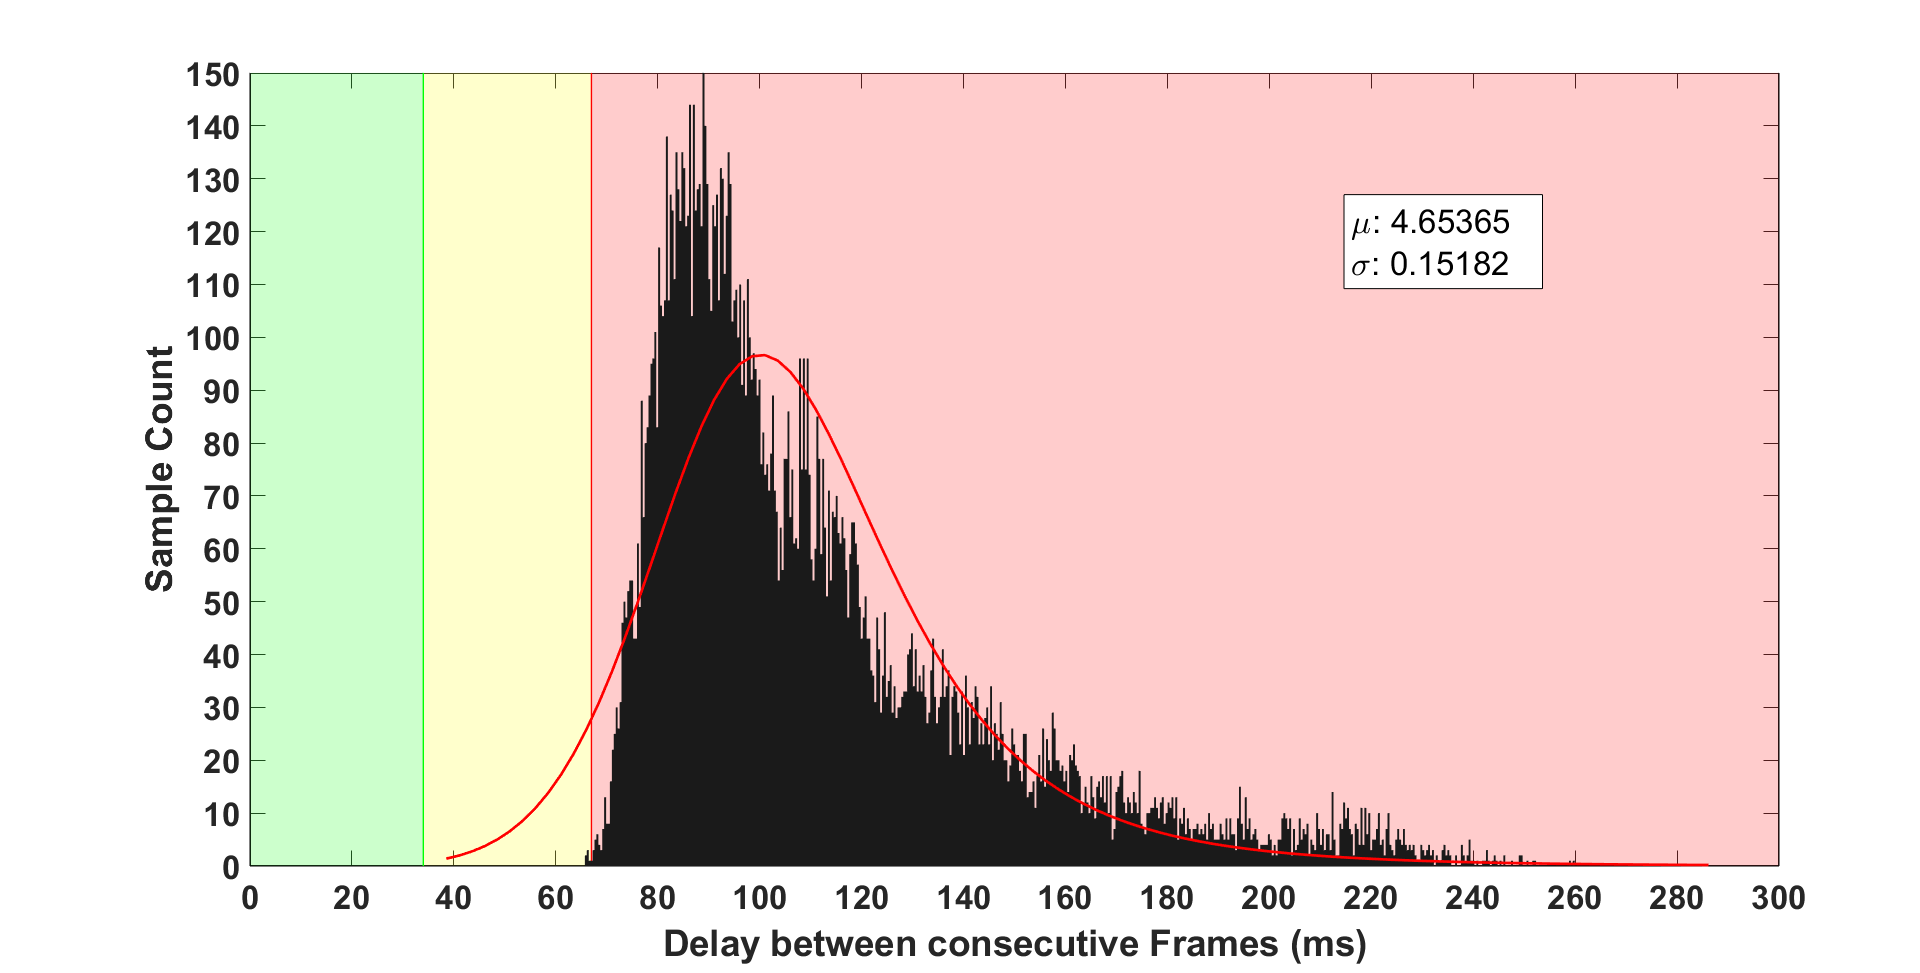
\includegraphics[width=\textwidth]{figures/graphs/dist_cmrcnn_resnet50.png}
\end{frame}

\begin{frame}{Processing Time Distribution YOLACT MobileNetV2}
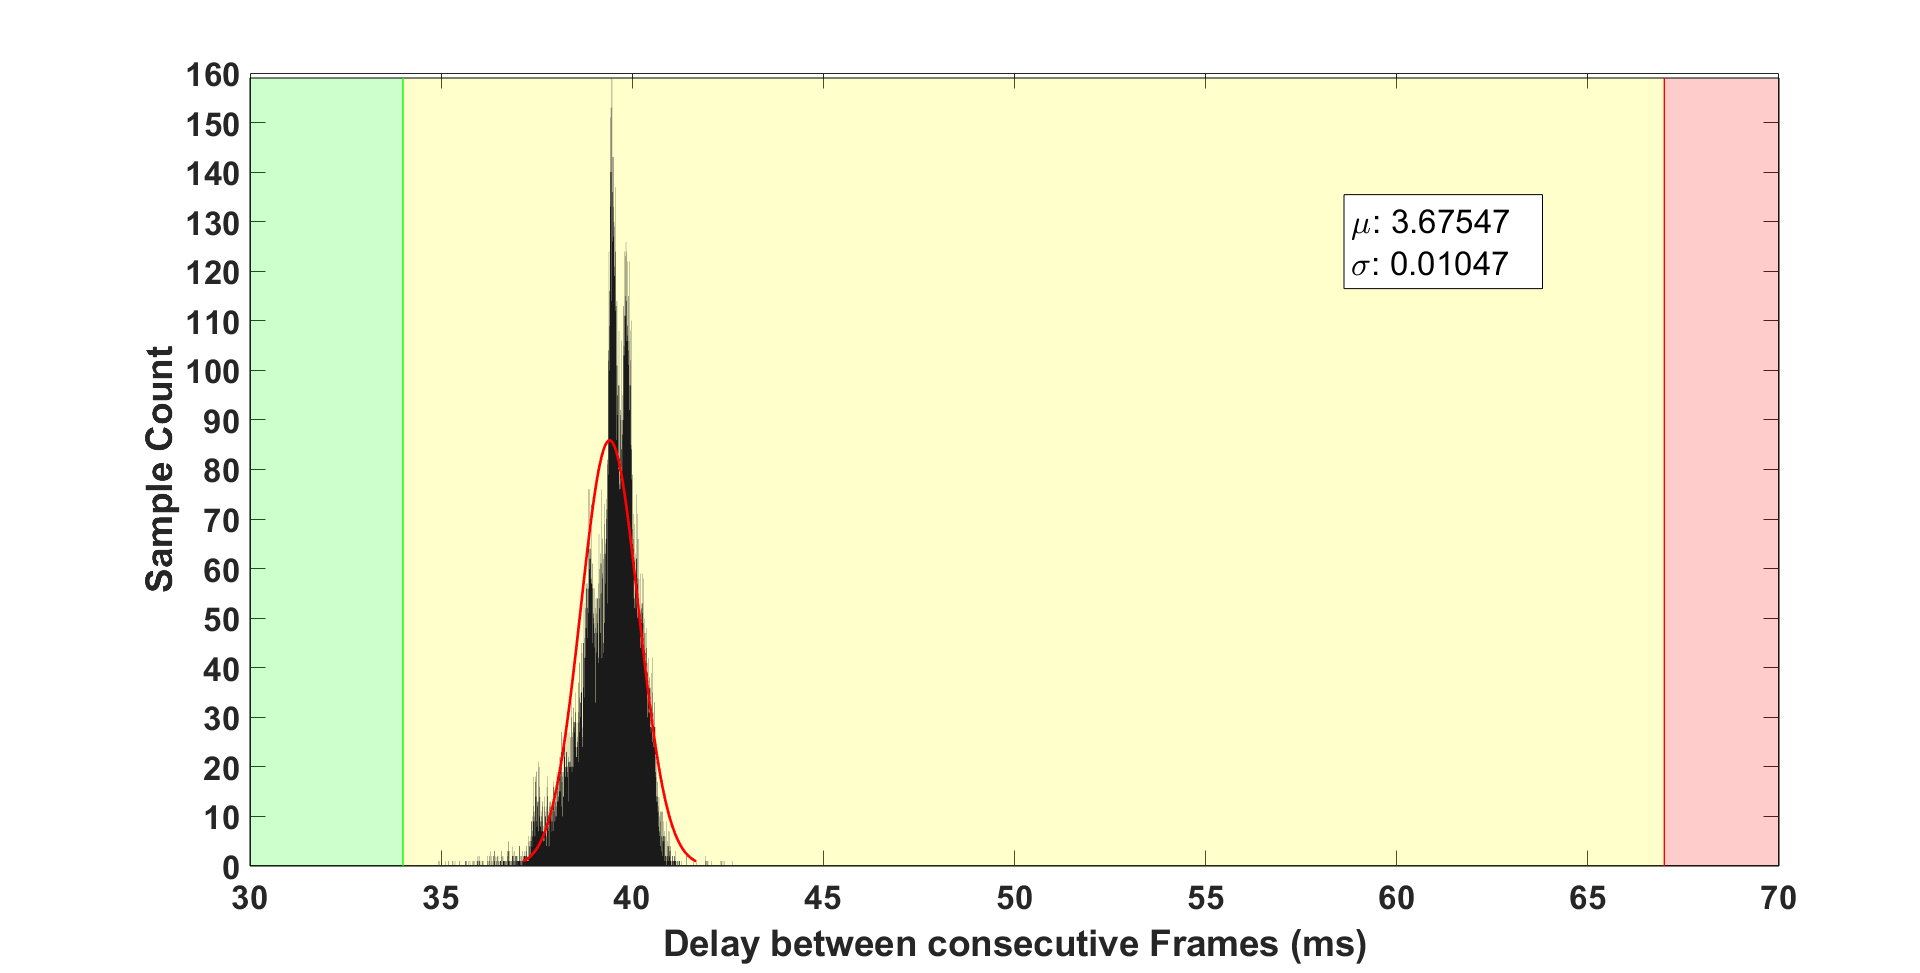
\includegraphics[width=\textwidth]{figures/graphs/dist_yolact_mobilenetv2.png}
\end{frame}

\begin{frame}{Stress Processing Time Distribution YOLACT ResNet50}
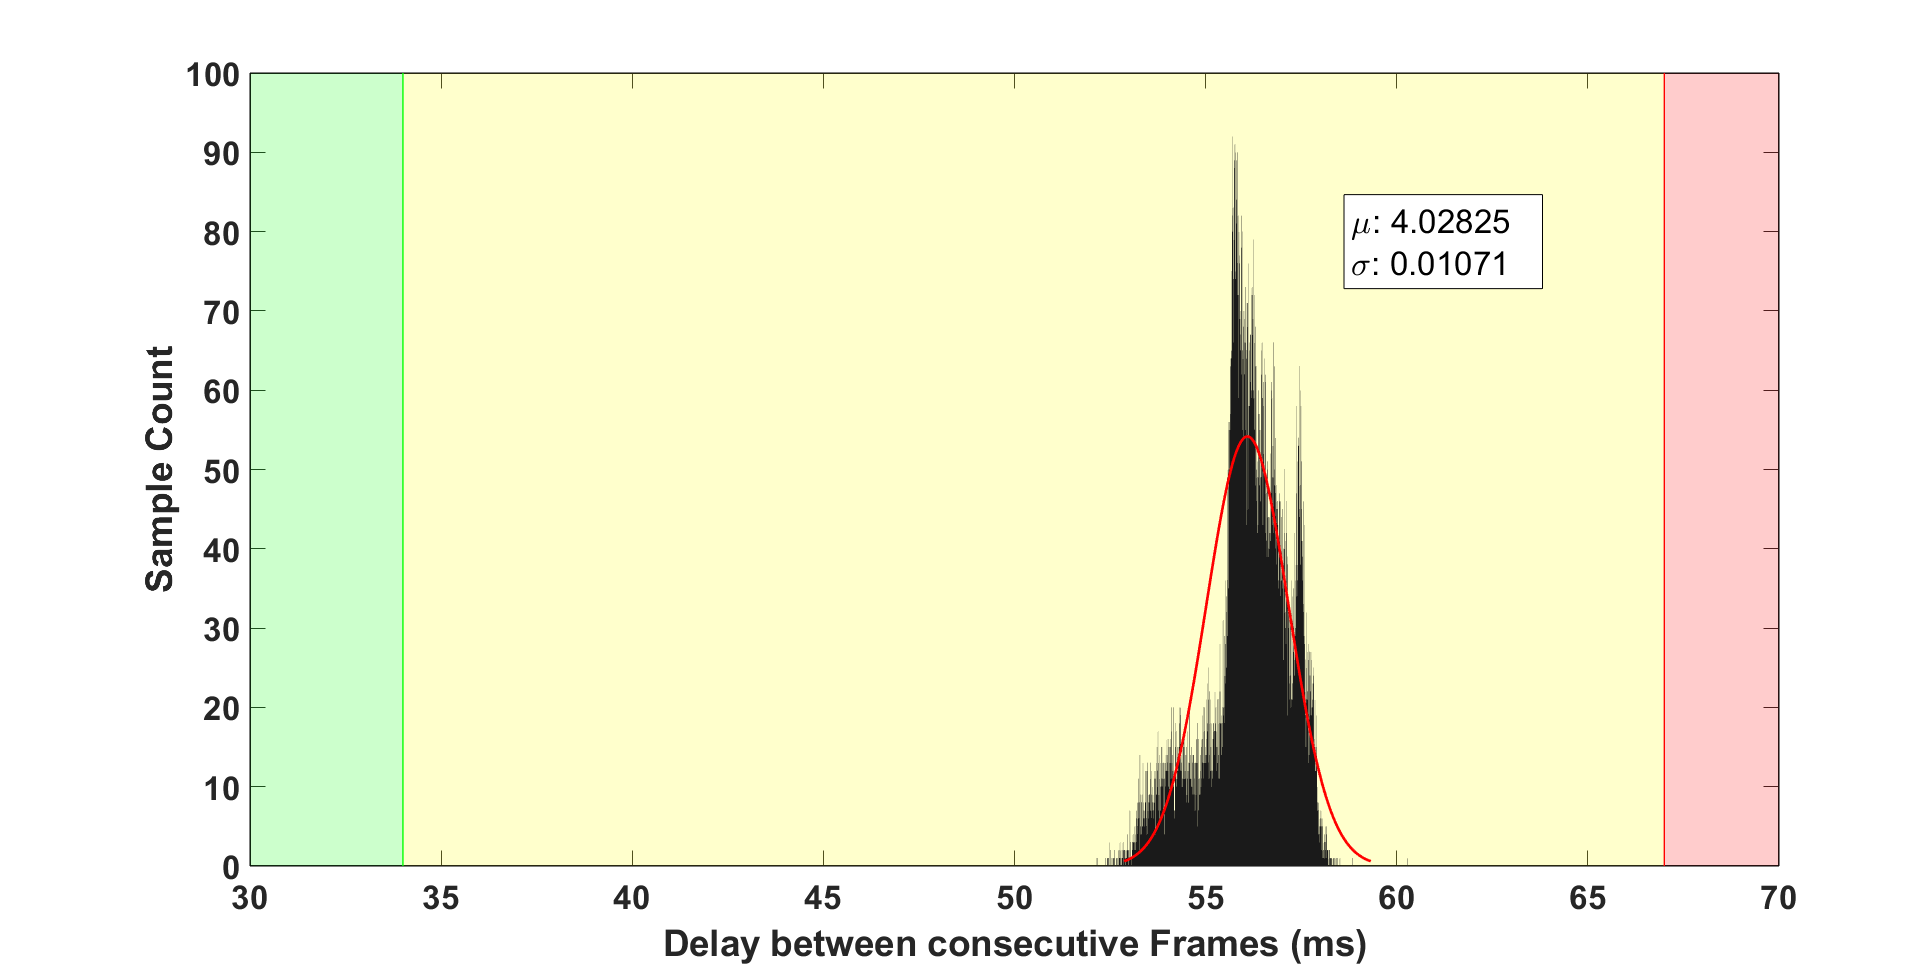
\includegraphics[width=\textwidth]{figures/graphs/dist_yolact_resnet50.png}
\end{frame}

\section{Stress Processing Time}

\begin{frame}{Stress Processing Time I}
\begin{table}[h]
    \begin{tabular}{ll | ccc}
        \toprule
        \multirow{2}{*}{Network}        & \multicolumn{1}{l}{\multirow{2}{*}{Backbone}}  & $Median$  & $Mean$    & $Var$     \\
        \multirow{1}{*}{}               & \multicolumn{1}{l}{\multirow{1}{*}{}}  			& $[ms]$  	& $[ms]$    & 		    \\
        \midrule
        \multirow{2}{*}{Cascade M-RCNN} & ResNet50                      & 1336.9    & 1214.6    & 226690.0 \\
        \multirow{1}{*}{}               & MobileNetV2                   & 1097.5    & 1025.7    & 111690.0  \\
        \midrule
        \multirow{2}{*}{YOLACT}         & ResNet50                      & 182.26    & \textbf{166.61}    & 4583.5   \\
        \multirow{1}{*}{}               & MobileNetV2                   & \textbf{181.2}     & 170.21    & \textbf{4281}\\
        \bottomrule
    \end{tabular}
\end{table}
\end{frame}

\begin{frame}{Stress Processing Time II}
\begin{table}[h]
    \begin{tabular}{ll | cc}
        \toprule
        \multirow{2}{*}{Network}        & \multicolumn{1}{l}{\multirow{2}{*}{Backbone}} & $Min$     & $Max$     \\
        \multirow{1}{*}{}               & \multicolumn{1}{l}{\multirow{1}{*}{}}  			& $[ms]$    & $[ms]$     \\
        \midrule
        \multirow{2}{*}{Cascade M-RCNN} & ResNet50                      & 536.81    & 4090.5    \\
        \multirow{1}{*}{}               & MobileNetV2                   & 502.43    & 3175.2    \\
        \midrule
        \multirow{2}{*}{YOLACT}         & ResNet50                       & \textbf{65.118}    & \textbf{880.47}    \\
        \multirow{1}{*}{}               & MobileNetV2                    & 66.392    & 1063      \\
        \bottomrule
    \end{tabular}
\end{table}
\end{frame}

\begin{frame}{Stress Processing Time Distribution CMRCNN MobileNetV2}
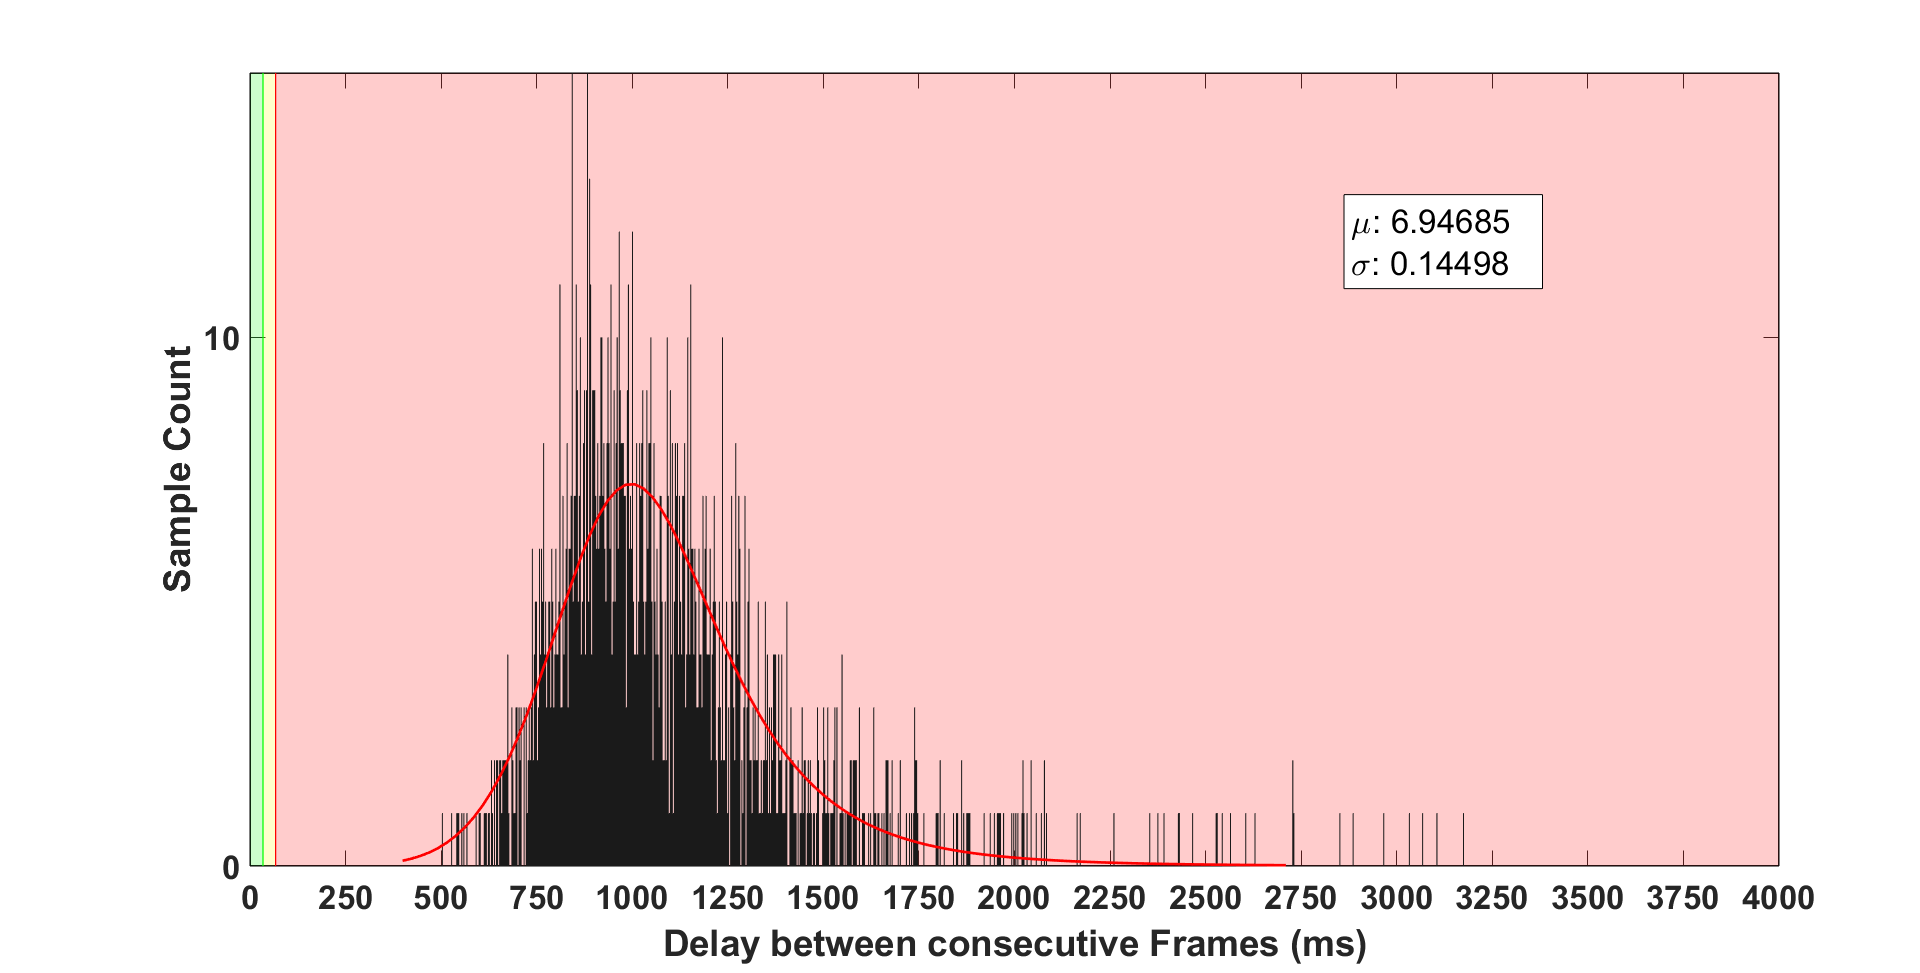
\includegraphics[width=\textwidth]{figures/graphs/dist_stress_cmrcnn_mobilenetv2.png}
\end{frame}

\begin{frame}{Stress Processing Time Distribution CMRCNN ResNet50}
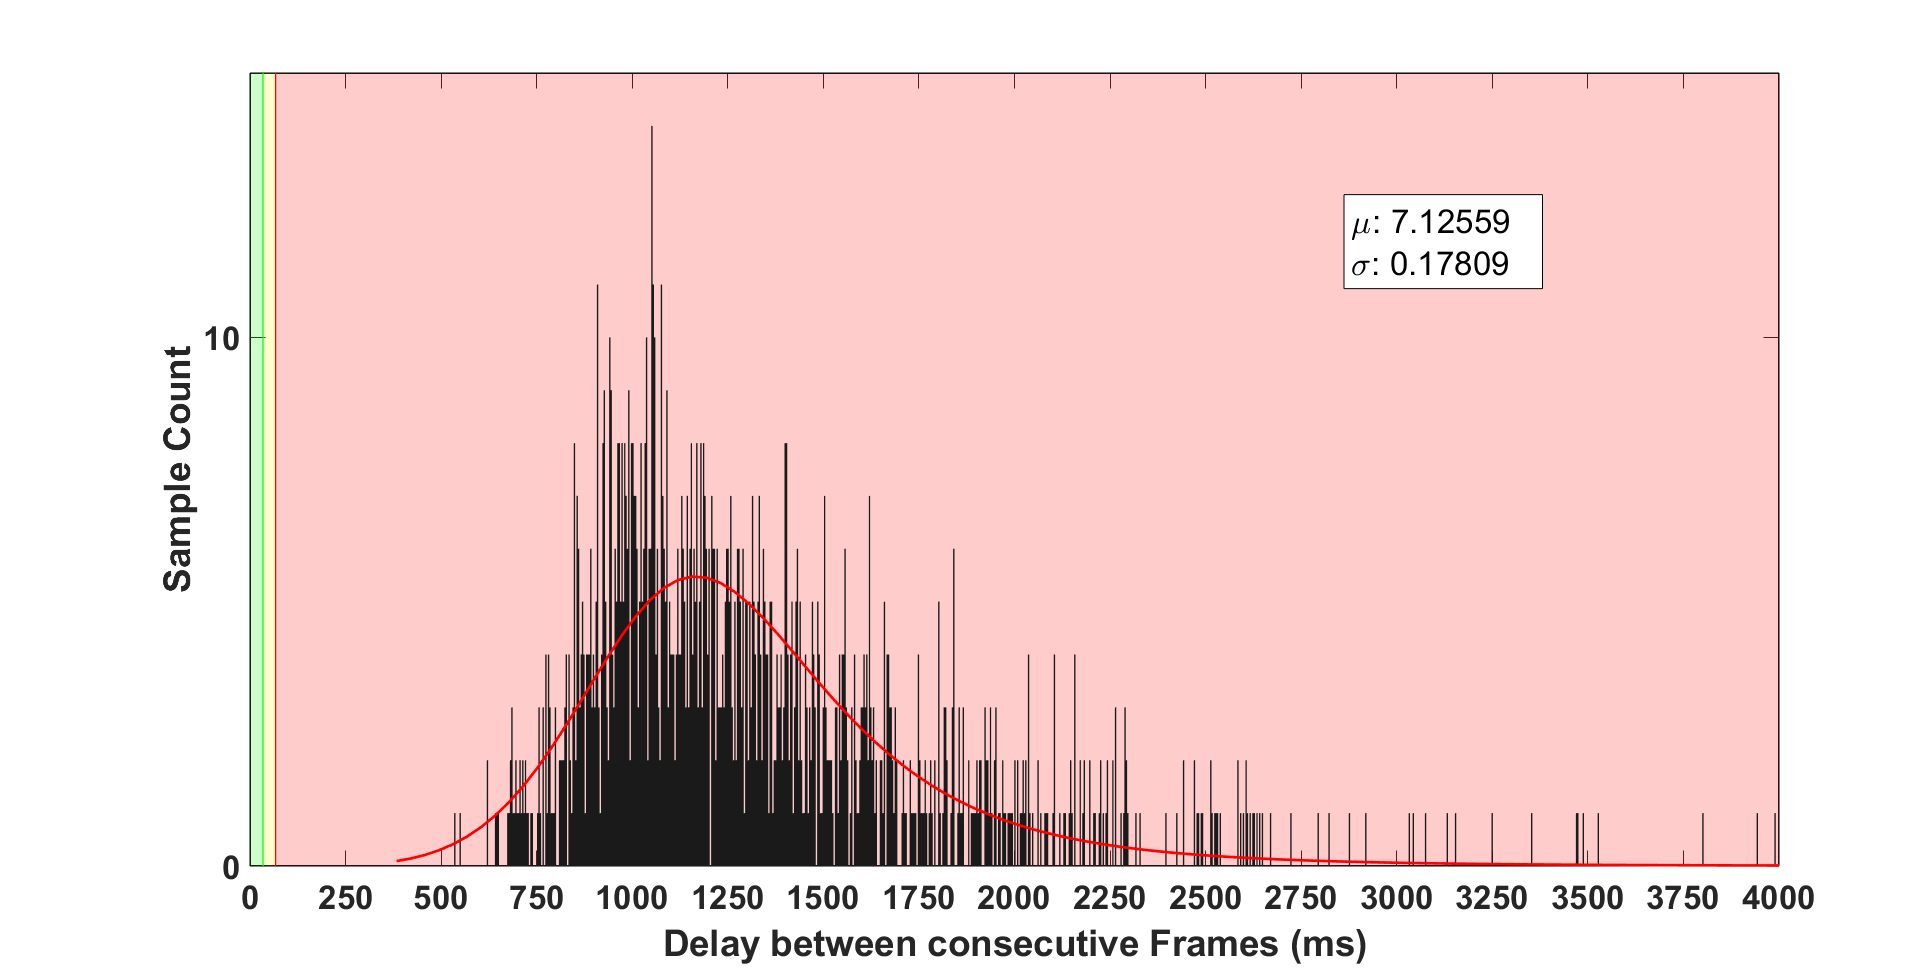
\includegraphics[width=\textwidth]{figures/graphs/dist_stress_cmrcnn_resnet50.png}
\end{frame}

\begin{frame}{Stress Processing Time Distribution YOLACT MobileNetV2}
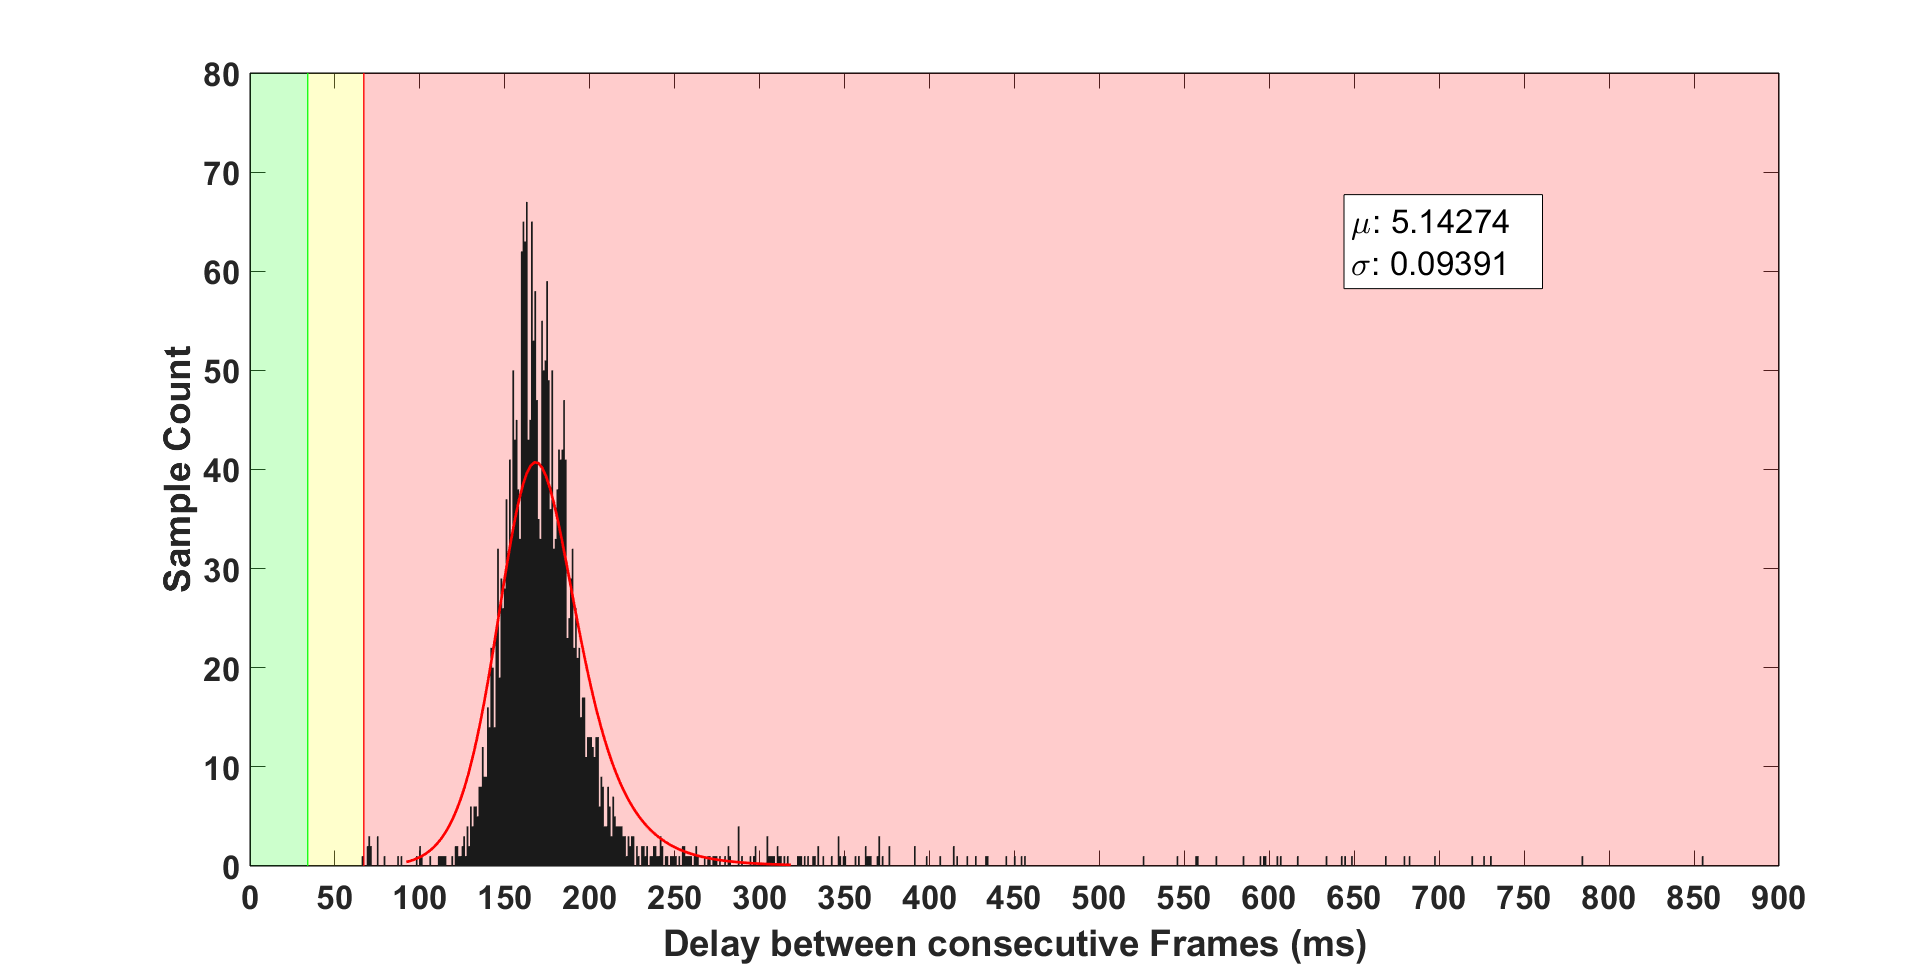
\includegraphics[width=\textwidth]{figures/graphs/dist_stress_yolact_mobilenetv2.png}
\end{frame}

\begin{frame}{Stress Processing Time Distribution YOLACT ResNet50}
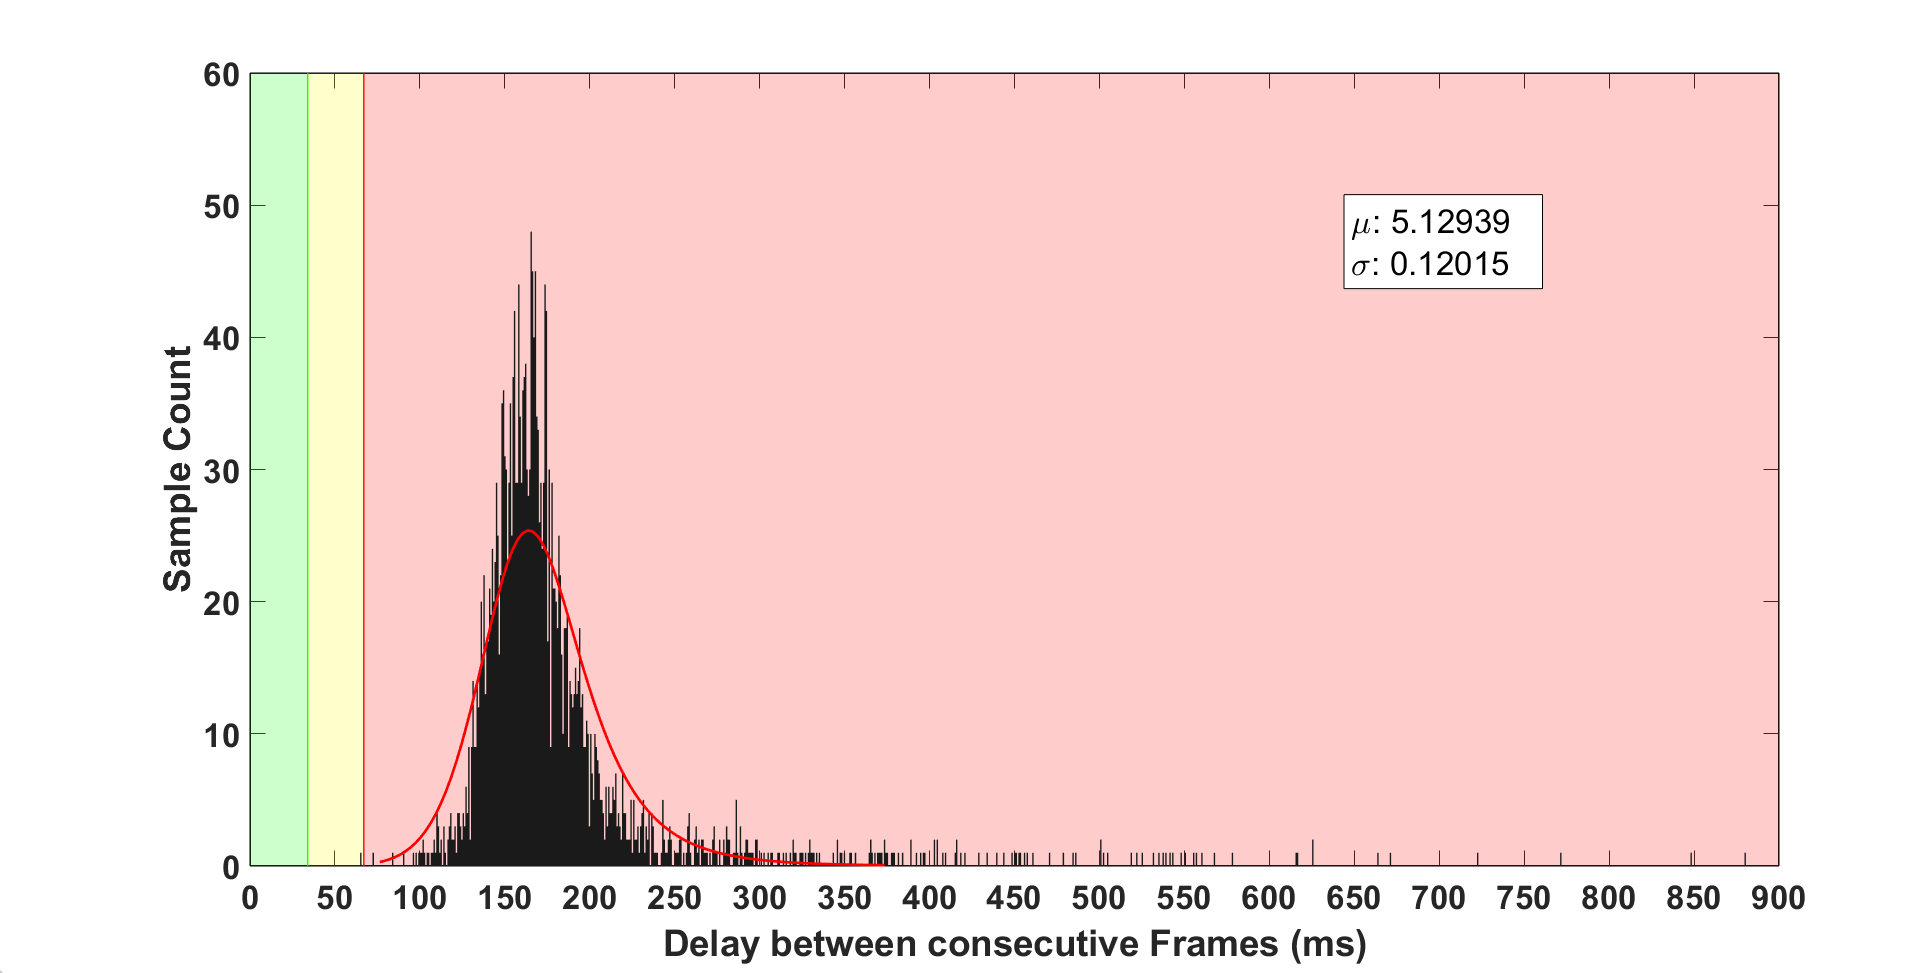
\includegraphics[width=\textwidth]{figures/graphs/dist_stress_yolact_resnet50.png}
\end{frame}

\section{Autocorrelations}

\begin{frame}{Autocorr CMRCNN MobileNetV2}
    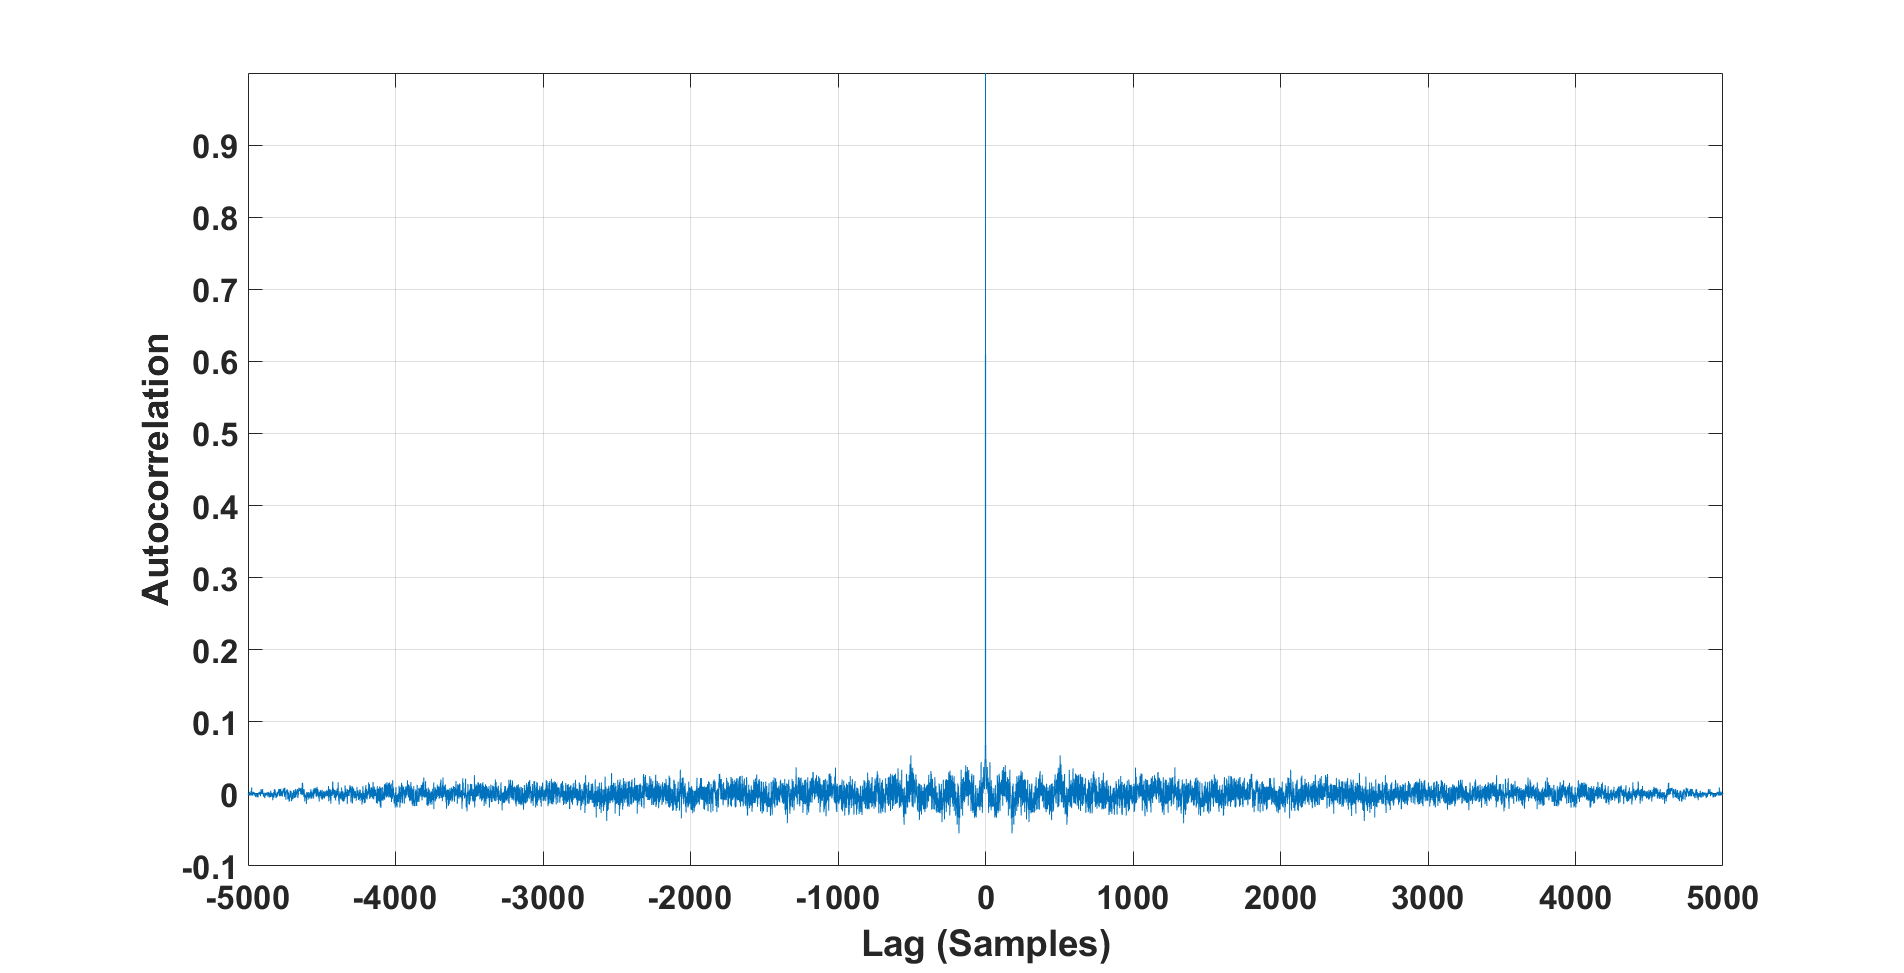
\includegraphics[width=\textwidth]{figures/graphs/autocorr_cmrcnn_mobilenetv2.png}
\end{frame}

\begin{frame}{Autocorr CMRCNN ResNet18}
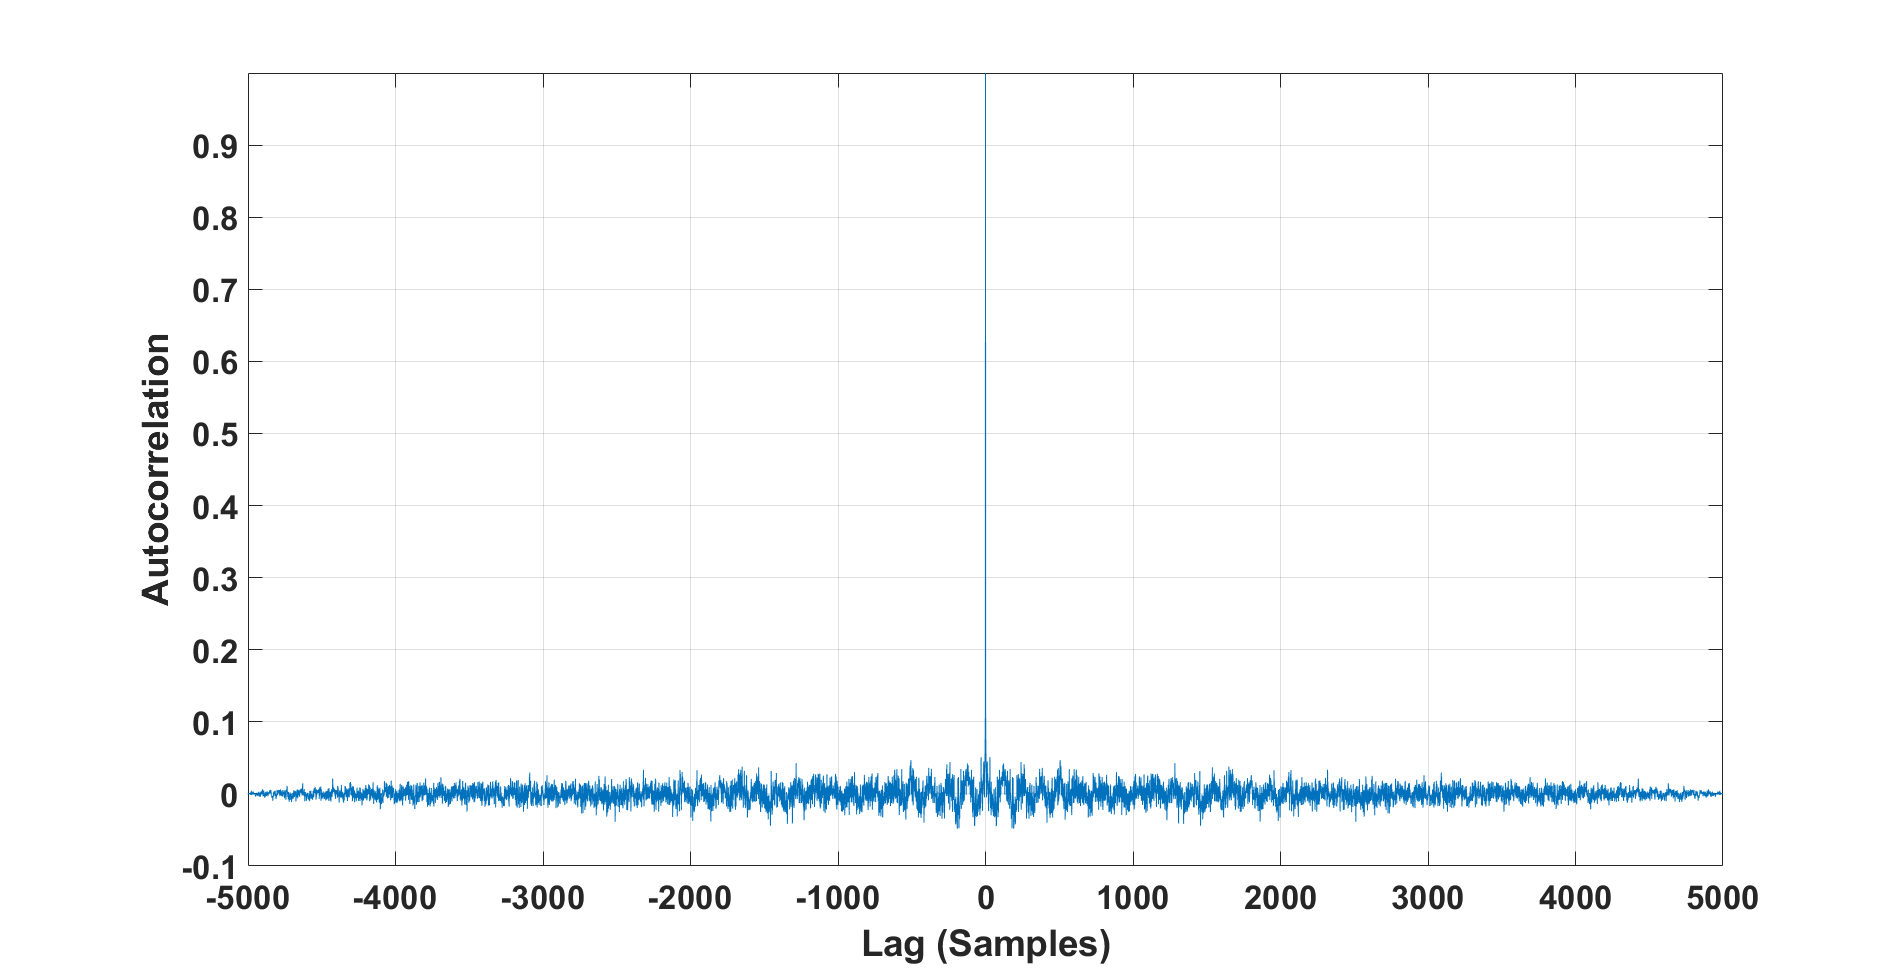
\includegraphics[width=\textwidth]{figures/graphs/autocorr_cmrcnn_resnet18.png}
\end{frame}

\begin{frame}{Autocorr CMRCNN ResNet50}
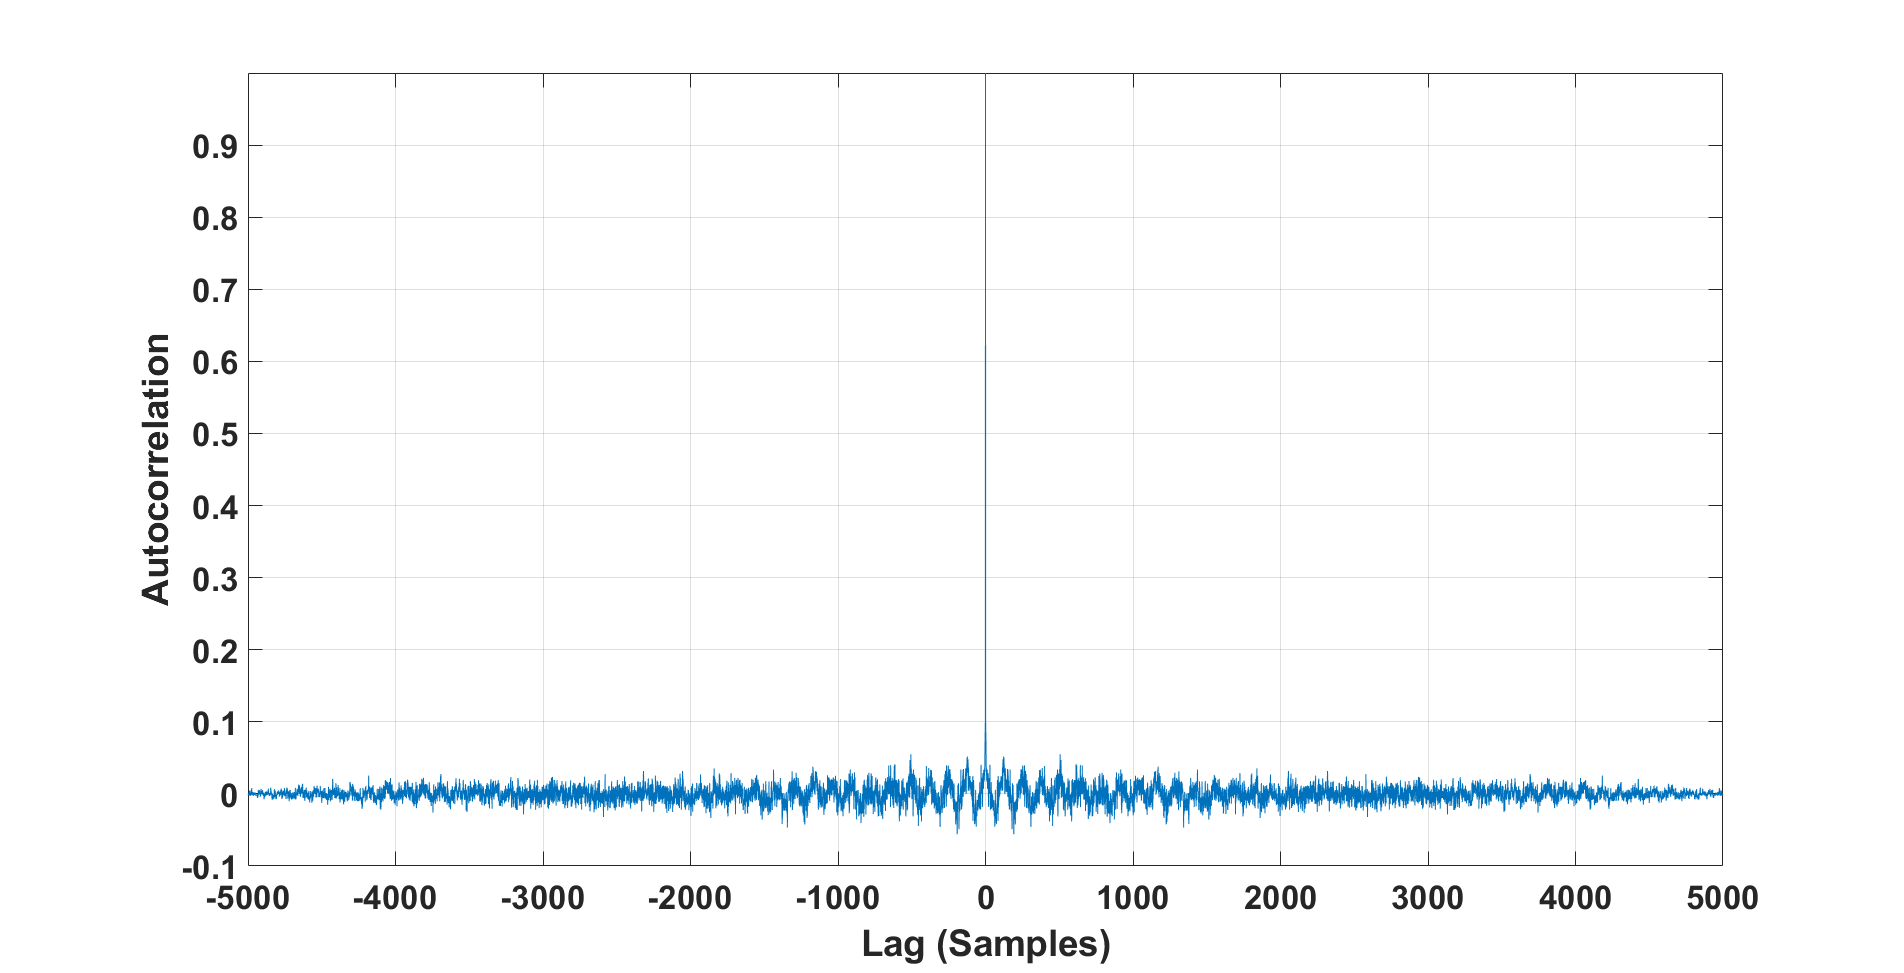
\includegraphics[width=\textwidth]{figures/graphs/autocorr_cmrcnn_resnet50.png}
\end{frame}

\begin{frame}{Autocorr YOLACT MobileNetV2}
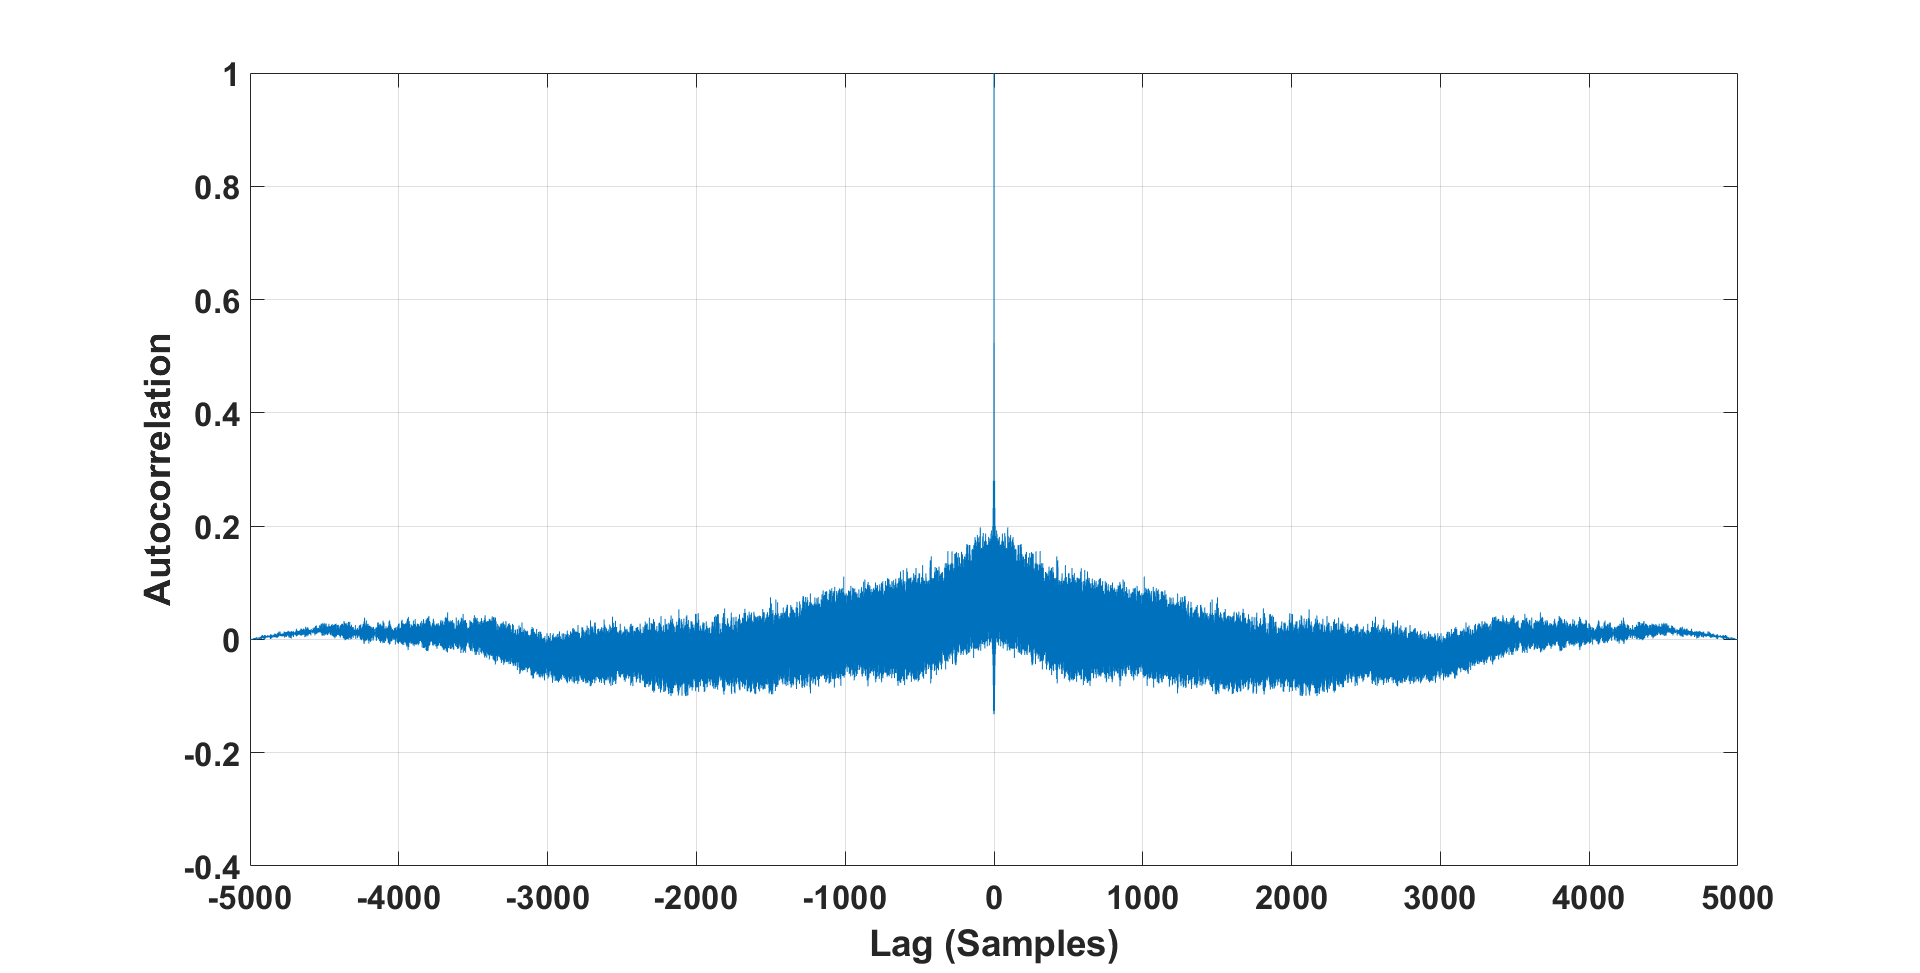
\includegraphics[width=\textwidth]{figures/graphs/autocorr_yolact_mobilenetv2.png}
\end{frame}

\begin{frame}{Autocorr YOLACT ResNet50}
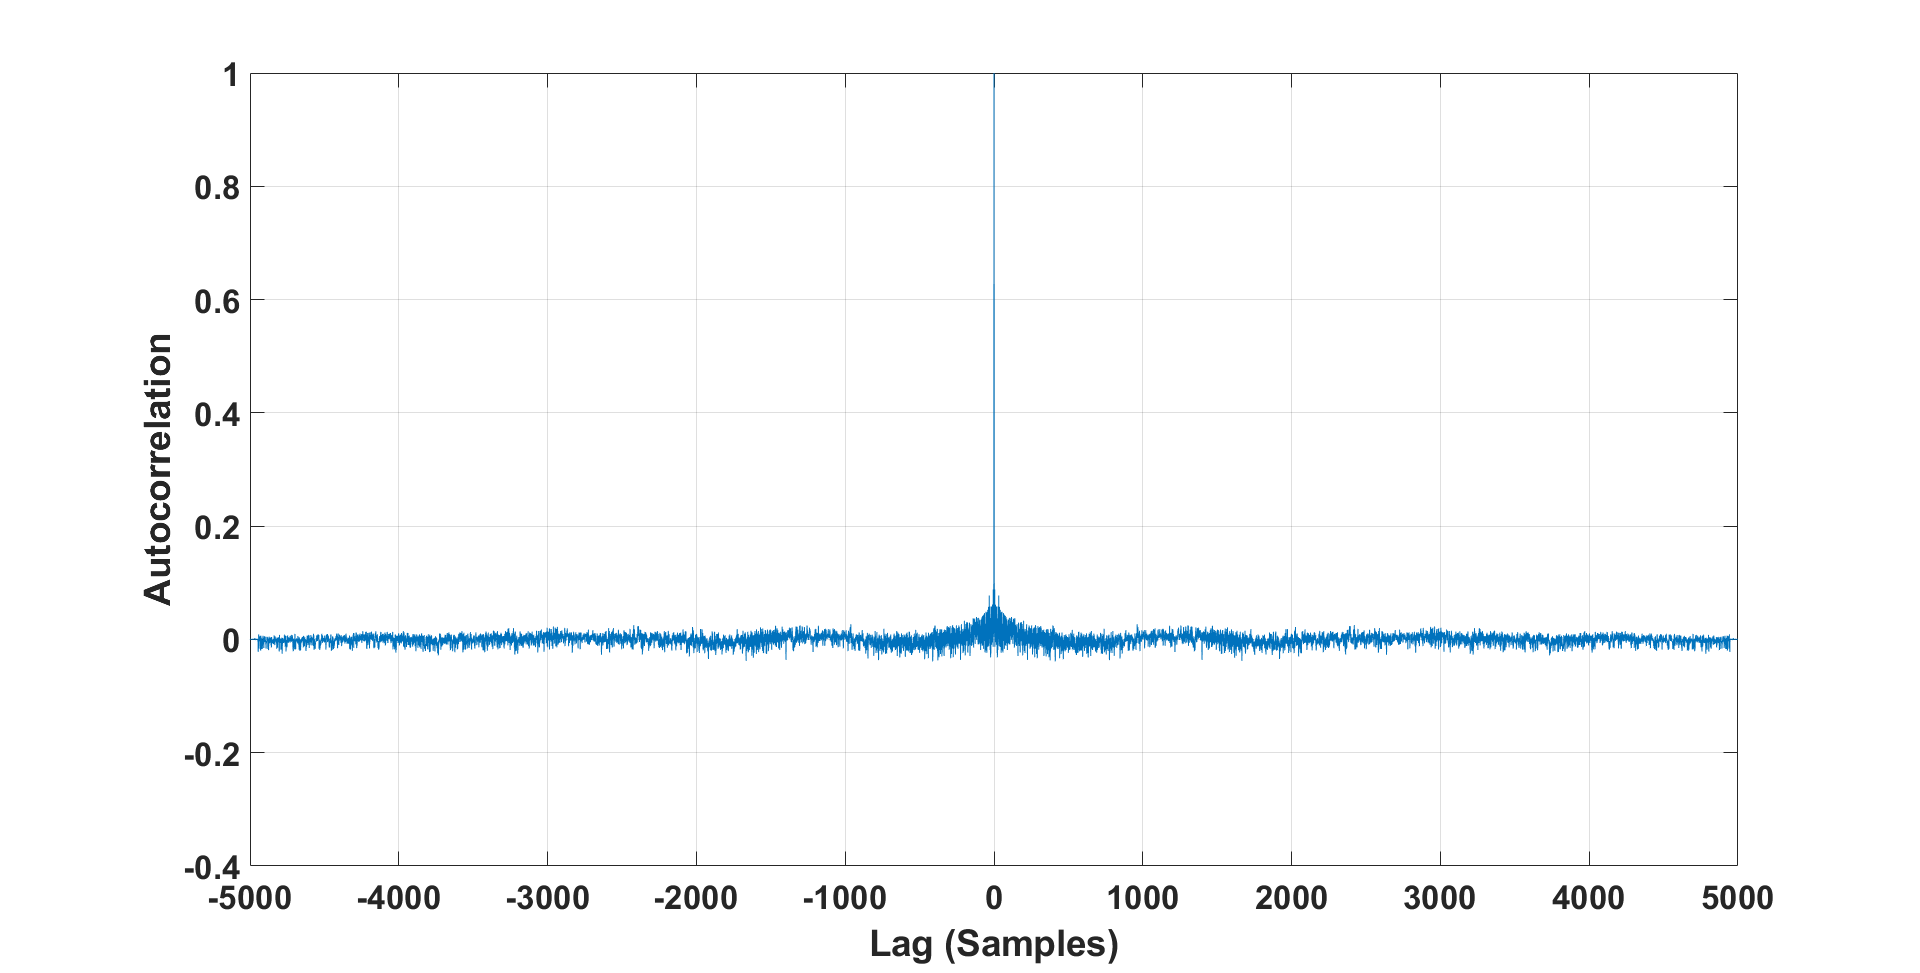
\includegraphics[width=\textwidth]{figures/graphs/autocorr_yolact_resnet50.png}
\end{frame}

\section{Datasets}
\begin{frame}{Dataset Intervals}

    \begin{table}[H]
        \centering
        \begin{tabular}{l c c}
            \hline
            Size-Class      & Area intervals ($\text{Pixel}^2$)     & Pixel count intervals (Pixel)     \\
            \hline
            All & $[0\%, 100\%]$ & $[0\%, 100\%]$ \\
            Small & $[0\%, 0.0033\%)$ & $[0\%, 0.057\%)$ \\
            Medium & $[0.0033\%, 0.03\%)$ & $[0.057\%, 0.173\%)$ \\
            Large & $[0.03\%, 100\%]$ & $[0.173\%, 100\%]$ \\
            \hline
        \end{tabular}
    \end{table}
\end{frame}

\begin{frame}{Dataset Properties}
\begin{table}[h]
    \centering
    \resizebox{\textwidth}{!}{%
    \begin{tabular}{l l | c | c | c c c}
        \hline
        \multicolumn{2}{c}{}						& \multicolumn{1}{c}{\multirow{2}{*}{FAT}} 	& \multicolumn{1}{c}{\multirow{2}{*}{YCB}}& \multicolumn{3}{c}{COCO} 										\\
        \multicolumn{2}{c}{}						& \multicolumn{1}{c}{}            			& \multicolumn{1}{c}{}	& \multicolumn{1}{c}{}     	& Indoor 0.02 		& \multicolumn{1}{c}{Indoor 0.10}	\\
        \hline
        Classes								&   	& 21             							& 21    				& 80             			& 41        		& 41       	 						\\
        \hline
        \multirow{2}{*}{Images}				& train &  55000 									& 11356					& 118287 					& 33092 			& 11293 							\\
        & val 	&  5000   									& 2079					& 5000  					& 1404     			& 515      							\\
        \hline
        \multirow{2}{*}{Annotations}		& train &  274793 									& 51366					& 860001 					& 12334				& 21386	 							\\
        & val 	&  24653 									& 9881					& 36781						& 5269    			& 965    							\\
        \hline
        \multicolumn{2}{c|}{Size Percentages}		&											&						&							&					&									\\
        \hline
        \multirow{2}{*}{Small}				& train & $20.41 \%$ 								& $1.12 \%$				& $41.43 \%$ 				& $8.68 \%$			& $1.74 \%$	 						\\
        & val 	& $19.82 \%$ 								& $0.1 \%$				& $41.63 \%$				& $8.97 \%$  		& $1.86 \%$    						\\
        \multirow{2}{*}{Medium}				& train & $68.64 \%$ 								& $31.75 \%$			& $34.32 \%$ 				& $42.41 \%$		& $10.05 \%$	 					\\
        & val 	& $69.52 \%$ 								& $25.91 \%$			& $34.17 \%$				& $42.58 \%$    	& $9.53 \%$    						\\
        \multirow{2}{*}{Large}				& train & $10.93 \%$ 								& $67.12 \%$			& $24.24 \%$ 				& $48.90 \%$		& $88.20 \%$						\\
        & val 	& $10.65 \%$ 								& $73.97 \%$			& $24.18 \%$				& $48.43 \%$ 		& $88.6 \%$    						\\
        \hline
    \end{tabular}
}
\end{table}
\end{frame}

\backupend

\end{document}
\grid
